% section | subsection | subsubsection | paragraph | subparagraph | verbatim | enumerate | item

% Just let it be an Article bro
\documentclass{article}

% Cover Metadata
\title{Coding Interview Preparation}
\date{22 Nov 2025}
\author{Maulana Hafidz Ismail}

% Equation Setup
\usepackage{amsmath}

% Image Setup
\usepackage{graphicx}
\usepackage{float}

% Link Setup
\usepackage{hyperref}

% Highlighting Setup
\usepackage{soul}
\usepackage{xcolor}
\sethlcolor{red!30}
\newcommand{\hlblue}[1]{\sethlcolor{cyan!30}\hl{#1}\sethlcolor{yellow}}

% Line Width
\sloppy
\setlength{\emergencystretch}{3em}
\hbadness=99999

% Code Syntax Setup
\usepackage{listings}
\usepackage{xcolor} % untuk warna
\lstset{
basicstyle=\ttfamily\small,
frame=single,
breaklines=true,
backgroundcolor=\color{gray!10},
keywordstyle=\color{blue},
commentstyle=\color{gray},
stringstyle=\color{red},
tabsize=2,
captionpos=b
}

% Start of the Article
\begin{document}

% Cover Page
\pagenumbering{gobble}
\maketitle
\newpage

% Table of Content Page
\tableofcontents
\newpage
\pagenumbering{arabic}

% Main Content
\section{Pengenalan ke Interview Coding}
\subsection{Proses-proses Interview}
\subsubsection{Proses Pengajuan Lamaran}
\begin{itemize}
    \item Resume Screening: Proses di mana perekrut menilai resume dan pengalaman kerja kandidat untuk menentukan kesesuaian dengan posisi yang dilamar.
    \item Interview with Recruiter: Pertemuan antara kandidat dan perekrut untuk mendiskusikan keterampilan dan pengalaman, serta memastikan kecocokan untuk peran.
\end{itemize}

\subsubsection{Proses Wawancara}
\begin{itemize}
    \item Technical Interviews: Wawancara yang berfokus pada kemampuan teknis kandidat, termasuk coding challenges dan pertanyaan tentang algoritma dan data structures.
    \item Behavioral Interviews: Wawancara yang mengeksplorasi bagaimana kandidat berkolaborasi dan menyelesaikan masalah dalam situasi kerja.
\end{itemize}

\subsubsection{Proses Kalibrasi}
\begin{itemize}
    \item Discussion of Candidate Performance: Tim yang terlibat dalam wawancara berkumpul untuk mendiskusikan kinerja kandidat dan memutuskan apakah akan memberikan tawaran pekerjaan.
    \item Boot Camp Process: Proses pelatihan bagi kandidat yang diterima untuk mempelajari cara kerja di perusahaan dan memilih tim yang diinginkan.
\end{itemize}

\subsection{Persiapan untuk Sukses}
\begin{itemize}
    \item Technical Interview: Wawancara di mana Anda menunjukkan kemampuan teknis dan soft skills yang sesuai dengan perusahaan.
    \item Soft Skills: Kemampuan sosial seperti komunikasi yang jelas dan etika kerja yang baik.
\end{itemize}

\subsection{Langkah-langkah dalam Wawancara Teknis}
\begin{itemize}
    \item Solve the Problem Conceptually First: Sebelum menulis kode, pastikan Anda memahami pertanyaan dengan jelas. Gunakan whiteboard untuk mencatat poin-poin penting.
    \item Pseudocode: Menulis langkah-langkah solusi dalam bentuk teks yang menyerupai kode, membantu Anda merumuskan ide sebelum menulis kode sebenarnya.
\end{itemize}

\subsection{Menggunakan Alat yang Tepat}
\begin{itemize}
    \item Data Structure: Struktur yang digunakan untuk menyimpan dan mengorganisir data. Contoh: menggunakan dictionary untuk menghitung jumlah pasang kaus kaki berdasarkan warna.
    \item Algorithm: Langkah-langkah sistematis untuk menyelesaikan masalah. Penting untuk memahami algoritma dan cara visualisasinya.
\end{itemize}

\subsection{Optimasi Kode}
\begin{itemize}
    \item Time Complexity: Ukuran seberapa cepat solusi Anda dapat dijalankan.
    \item Space Complexity: Ukuran seberapa banyak memori yang digunakan oleh solusi Anda.
    \item DRY Principle (Don't Repeat Yourself): Prinsip untuk menghindari pengulangan kode, sehingga kode lebih efisien dan mudah dipelihara.
\end{itemize}

\subsection{Tipe-tipe interview}
\subsubsection{Screening}
Kontak pertama Anda dengan sebuah perusahaan akan berupa wawancara penyaringan. Seorang perekrut, setelah membaca lamaran Anda, biasanya akan mengatur panggilan telepon untuk membahas kesesuaian potensial Anda. Tahap ini bertujuan untuk menentukan apakah Anda benar-benar tertarik dengan posisi tersebut dan apakah Anda cocok dengan perusahaan. Ini adalah kesempatan yang baik bagi Anda, sebagai calon karyawan, untuk mempelajari lebih lanjut tentang posisi, perusahaan, dan proses perekrutan mereka. Beberapa pertanyaan yang baik untuk diajukan antara lain:
\begin{itemize}
    \item Apa peran yang dimaksud?
    \item Bahasa pemrograman apa yang biasanya digunakan oleh perusahaan?
    \item Bagaimana proses wawancara, jenis wawancara apa yang akan dilakukan, dan berapa banyak wawancara yang akan ada?
    \item Apa sifat proyek yang akan ditangani oleh peran yang diusulkan?
    \item Bagaimana komposisi tim yang biasanya ada?
    \item Siapa saja yang akan menjadi anggota panel wawancara, dan apa peran mereka di perusahaan?
\end{itemize}
Ingatlah bahwa pewawancara ingin memberikan Anda kesempatan untuk menyampaikan argumen yang meyakinkan mengapa Anda layak untuk dipekerjakan. Mereka seharusnya bersedia memberikan informasi apa pun yang dapat membantu Anda mempersiapkan diri dengan lebih baik.

Dari sudut pandang perusahaan, proses seleksi biasanya akan fokus pada keterampilan lunak atau interpersonal Anda. Tidak akan ada pertanyaan teknis, dan proses ini biasanya akan dilakukan oleh perwakilan Sumber Daya Manusia (SDM). Menampilkan diri dengan baik dan menunjukkan kemampuan sosial Anda, seperti mendengarkan dan menjawab pertanyaan, sangat penting.

\subsubsection{Quiz}
Ujian kuis adalah cara yang sangat sederhana untuk menentukan apakah seorang kandidat mampu mengkodekan. Biasanya, ujian ini dilakukan pada tahap awal proses wawancara dan berfungsi sebagai penyaring untuk mengurangi jumlah wawancara yang harus dilakukan oleh perusahaan. Anda tidak boleh mengharapkan pertanyaan yang mendalam atau panjang; tujuan utamanya adalah untuk menentukan apakah kandidat memiliki pemahaman yang baik tentang dasar-dasar pemrograman. Beberapa pertanyaan yang mungkin diajukan antara lain:
\begin{itemize}
    \item Bagaimana cara memeriksa nilai null dalam array menggunakan bahasa pemrograman pilihan Anda?
    \item Apa kompleksitas ruang untuk algoritma Quicksort?
    \item Struktur data apa yang akan Anda gunakan untuk menyimpan daftar kunci dan nilai?
    \item Apa yang dimaksud dengan tabrakan (collision) dalam hashing?
    \item Apa sintaksis untuk memilih nama kolom menggunakan SQL?
    \item Proses pengujian apa yang Anda kenal?
\end{itemize}
Pertanyaan-pertanyaan tersebut akan bersifat spesifik untuk posisi yang dilamar, sehingga isi pertanyaannya dapat bervariasi. Namun, pertanyaan-pertanyaan tersebut harus dijawab dengan jawaban yang ringkas dan langsung. Saat mempersiapkan diri untuk wawancara, disarankan untuk mengidentifikasi bahasa pemrograman apa yang digunakan oleh perusahaan dan informasi teknis lainnya yang dapat diperoleh dari deskripsi pekerjaan dan proses seleksi awal.

\subsubsection{Online Coding Assignment}
Anda mungkin diminta untuk menyelesaikan tugas pemrograman online, tergantung pada posisi yang Anda lamar. Hal ini umumnya dilakukan sebelum wawancara teknis, karena hasilnya dapat digunakan sebagai bahan pembahasan selama wawancara selanjutnya. Namun, tugas tersebut juga dapat dilakukan setelah wawancara teknis yang sukses untuk membandingkan kandidat.

Langkah ini memungkinkan Anda untuk mendekati dan menyelesaikan tugas yang jelas didefinisikan dalam lingkungan yang tidak menekan. Mirip dengan tingkat kesulitan kuis, ini adalah langkah penyaringan untuk memastikan Anda dapat bekerja dengan teknologi target dan memahami dasar-dasarnya, seperti loop, Boolean, pengecekan, dan sebagainya. Beberapa tugas pemrograman mungkin dibatasi waktu; dalam situasi ini, Anda akan memiliki akses ke Google dan bahan referensi lainnya.

\subsubsection{The Technical Interview}
Ini juga disebut sebagai tantangan pemrograman. Biasanya, hal ini akan dilakukan setelah tahap seleksi awal. Tantangan ini dapat dilakukan secara virtual atau tatap muka. Pewawancara akan memberikan Anda masalah yang menantang dan memberi Anda waktu singkat untuk menyelesaikannya. Selalu lebih baik untuk mengutarakan pemikiran Anda secara lisan saat menghadapi tantangan tersebut. Misalnya, sebelum memutuskan antara dua struktur data, jelaskan mengapa Anda merasa salah satunya lebih cocok untuk tugas tersebut. Manfaatkan kesempatan ini untuk menunjukkan pemahaman umum Anda tentang topik dan keahlian khusus yang relevan dengan tugas.

Tingkat kesulitan wawancara teknis seharusnya rendah. Pewawancara menyadari bahwa Anda tidak memiliki akses ke Google dan mungkin harus menghafal beberapa sintaks yang diperlukan. Sebaliknya, wawancara ini dirancang untuk menunjukkan kemampuan pemecahan masalah Anda. Beberapa wawancara teknis mungkin dilakukan menggunakan pseudocode. Selain itu, wawancara teknis memungkinkan rekan kerja masa depan untuk menilai kemampuan Anda dalam berargumen dengan kode. Mereka sering kali mencakup prompt singkat dan spesifik seperti:
\begin{itemize}
    \item Bagaimana Anda menjelaskan teknologi X kepada orang yang tidak memiliki latar belakang teknis?
    \item Teknologi apa yang paling Anda sukai dan mengapa?
    \item Database apa saja yang pernah Anda gunakan?
    \item Ceritakan tentang tantangan teknis yang pernah Anda atasi dalam sebuah proyek.
    \item Proyek apa saja yang pernah Anda kerjakan di waktu luang Anda?
\end{itemize}

Ini adalah pertanyaan umum, dan wawancara teknis akan disesuaikan dengan peran spesifik. Namun, menyiapkan beberapa jawaban yang menggambarkan perjalanan Anda sebagai programmer adalah praktik yang baik. Tinjau proyek-proyek Anda dan jelaskan dengan jelas berbagai keputusan yang telah Anda ambil dan alasannya, terutama saat memilih satu teknologi daripada yang lain.

\subsubsection{The take-home assignment}
Jika Anda sampai sejauh ini, Anda sudah melakukan dengan sangat baik. Hal ini mungkin terjadi sebelum atau setelah wawancara teknis, karena pewawancara mungkin ingin mendiskusikan proses berpikir Anda terkait solusi yang Anda berikan sebelumnya dalam proses ini. Jika ada beberapa putaran wawancara untuk posisi ini, maka hal ini mungkin terjadi di antara dua wawancara teknis. Sebuah perusahaan tidak boleh meminta Anda untuk mengerjakan tugas di rumah kecuali mereka merasa Anda berpotensi cocok untuk posisi tersebut.

Anda akan diberikan beberapa hari untuk mengembangkan solusi untuk tantangan tersebut. Anda mungkin diminta untuk membangun aplikasi atau memecahkan masalah rute lalu lintas secara programatik. Tugas lain mungkin spesifik proyek, misalnya, jika Anda akan bekerja dengan pemrosesan gambar, Anda mungkin diminta untuk menunjukkan bahwa Anda dapat mendeteksi objek secara otomatis dalam aliran video.

\subsubsection{Top Tips}
Lakukan riset sebelum setiap wawancara dan tinjau setiap wawancara setelah selesai. Sebagian besar perusahaan senang memberikan umpan balik setelah wawancara Anda, jadi selalu mintalah hal ini dan gunakan poin-poin yang disampaikan sebagai titik awal untuk mempersiapkan diri dengan lebih baik untuk wawancara berikutnya. Ingat, latihan membuat sempurna.

\subsection{Kommunikasi Non-Verbal}
\begin{itemize}
    \item Punctuality: Datang tepat waktu, idealnya 10 menit sebelum wawancara, menunjukkan keseriusan dan kesiapan.
    \item Eye Contact: Mempertahankan kontak mata selama wawancara untuk menunjukkan perhatian dan keterlibatan.
\end{itemize}

\subsection{Komunikasi Verbal}
\begin{itemize}
    \item Clear and Concise Language: Gunakan bahasa yang jelas dan ringkas saat menjawab pertanyaan untuk menghindari kebingungan.
    \item STAR Method: Metode untuk menjawab pertanyaan wawancara dengan menyusun jawaban berdasarkan Situasi, Tugas, Aksi, dan Hasil.
\end{itemize}

\subsection{Jenis Wawancara}
\begin{itemize}
    \item Technical Interview: Wawancara di mana kandidat menunjukkan kemampuan teknis mereka melalui pertanyaan coding dan algoritma.
    \item Architecture Interview: Wawancara yang berfokus pada bagaimana membangun fitur end-to-end, termasuk pertimbangan tentang aliran data dan skalabilitas.
    \item Behavioral Interview: Wawancara yang mengeksplorasi pengalaman kandidat dalam bekerja dengan orang lain, tantangan yang dihadapi, dan proyek menarik yang telah dikerjakan.
\end{itemize}

\subsection{Persiapan untuk Wawancara}
\begin{itemize}
    \item Practice: Latihan dengan menjelaskan solusi saat menulis kode, termasuk pertimbangan tentang time complexity dan space complexity.
    \item Dress Code: Kenakan pakaian yang nyaman; tidak perlu formal seperti jas. T-shirt dan jeans sudah cukup.
    \item Communication: Penting untuk menjelaskan pemikiran saat coding, terutama jika mengalami kesulitan.
\end{itemize}

\subsection{Kualitas yang Dicari}
\begin{itemize}
    \item Enthusiasm: Kandidat yang menunjukkan semangat dan sikap positif lebih disukai.
    \item Feedback Reception: Kemampuan untuk menerima umpan balik dan berkolaborasi dalam menyelesaikan masalah adalah nilai tambah.
\end{itemize}

\subsection{Pseudocode}
\subsubsection{Kenapa menggunakan Pseudocode}
Pseudocode adalah langkah awal yang sah saat mulai merancang solusi. Pseudocode adalah representasi tingkat tinggi dari ide-ide yang ditulis dengan cara yang mirip dengan kode. Pada dasarnya, pseudocode dapat menjadi alat bantu untuk menyoroti bagi diri sendiri elemen-elemen apa yang harus termasuk dalam program.

Setiap baris akan memberi Anda kesempatan untuk berhenti sejenak dan mempertimbangkan apa yang diperlukan untuk mencapai hasil yang diinginkan. Saat menulis aplikasi, keputusan yang diambil pada langkah 3 dapat memengaruhi cara langkah 6 harus dikodekan. Setiap tahap memiliki unsur keterbatasan yang memengaruhi cara tahap berikutnya akan diselesaikan.

Pertimbangkan bahwa Anda sedang menulis aplikasi yang harus menyimpan data pada langkah 3. Anda memutuskan untuk menggunakan array sebelum melanjutkan. Pada langkah 6, Anda menyadari bahwa beberapa pencarian diperlukan untuk aplikasi tersebut. Saat menulis pseudocode, mudah untuk kembali ke langkah 3 dan mengubah struktur data menjadi sesuatu yang lebih kompatibel dengan langkah 6, seperti menggunakan kamus (dictionary) daripada array. Perubahan kecil dapat meningkatkan beban kerja jika implementasi sudah dimulai karena hal itu mengubah cara langkah 4 dan 5 beroperasi.

\subsubsection{Kapan harus menulis Pseudocode}
\begin{itemize}
    \item Sebagai pemula, saat merencanakan kemajuan yang direncanakan dalam pendekatan Anda.
    \item Sebagai programmer berpengalaman, saat berusaha mengatasi masalah yang kompleks.
    \item Jika Anda mencoba menjelaskan konsep kepada audiens yang berpengaruh, seperti tim atau klien potensial.
    \item Jika Anda memberikan petunjuk tentang pekerjaan Anda untuk programmer masa depan yang mungkin akan memelihara kode atau aplikasi yang Anda tulis.
    \item Dalam wawancara, saat menunjukkan kemampuan Anda untuk menganalisis dan memecahkan masalah.
\end{itemize}

\subsubsection{Bagaimana cara menulis Pseudocode}
Tidak ada satu cara baku untuk menulis pseudocode. Setiap organisasi mungkin memiliki standar tersendiri. Secara umum, dapat dikatakan bahwa pseudocode dapat dianggap sebagai representasi teks apa pun yang menggambarkan operasi suatu program.

Pertimbangkan cara mewakili tantangan FizzBuzz yang digunakan untuk menguji kemampuan kandidat dalam berlogika dalam kode:

\textit{Tulis program dalam bahasa pemrograman yang ditentukan yang mengiterasi angka dari 1 hingga 40. Cetak angka untuk setiap angka kecuali kelipatan tiga, dalam hal ini cetak Fizz. Untuk kelipatan lima, cetak Buzz, dan untuk kelipatan 3 dan 5, cetak FizzBuzz.}

Anda mungkin mulai dengan mewakili setiap persyaratan sebagai baris pseudocode:
\begin{figure}[H]
    \centering
    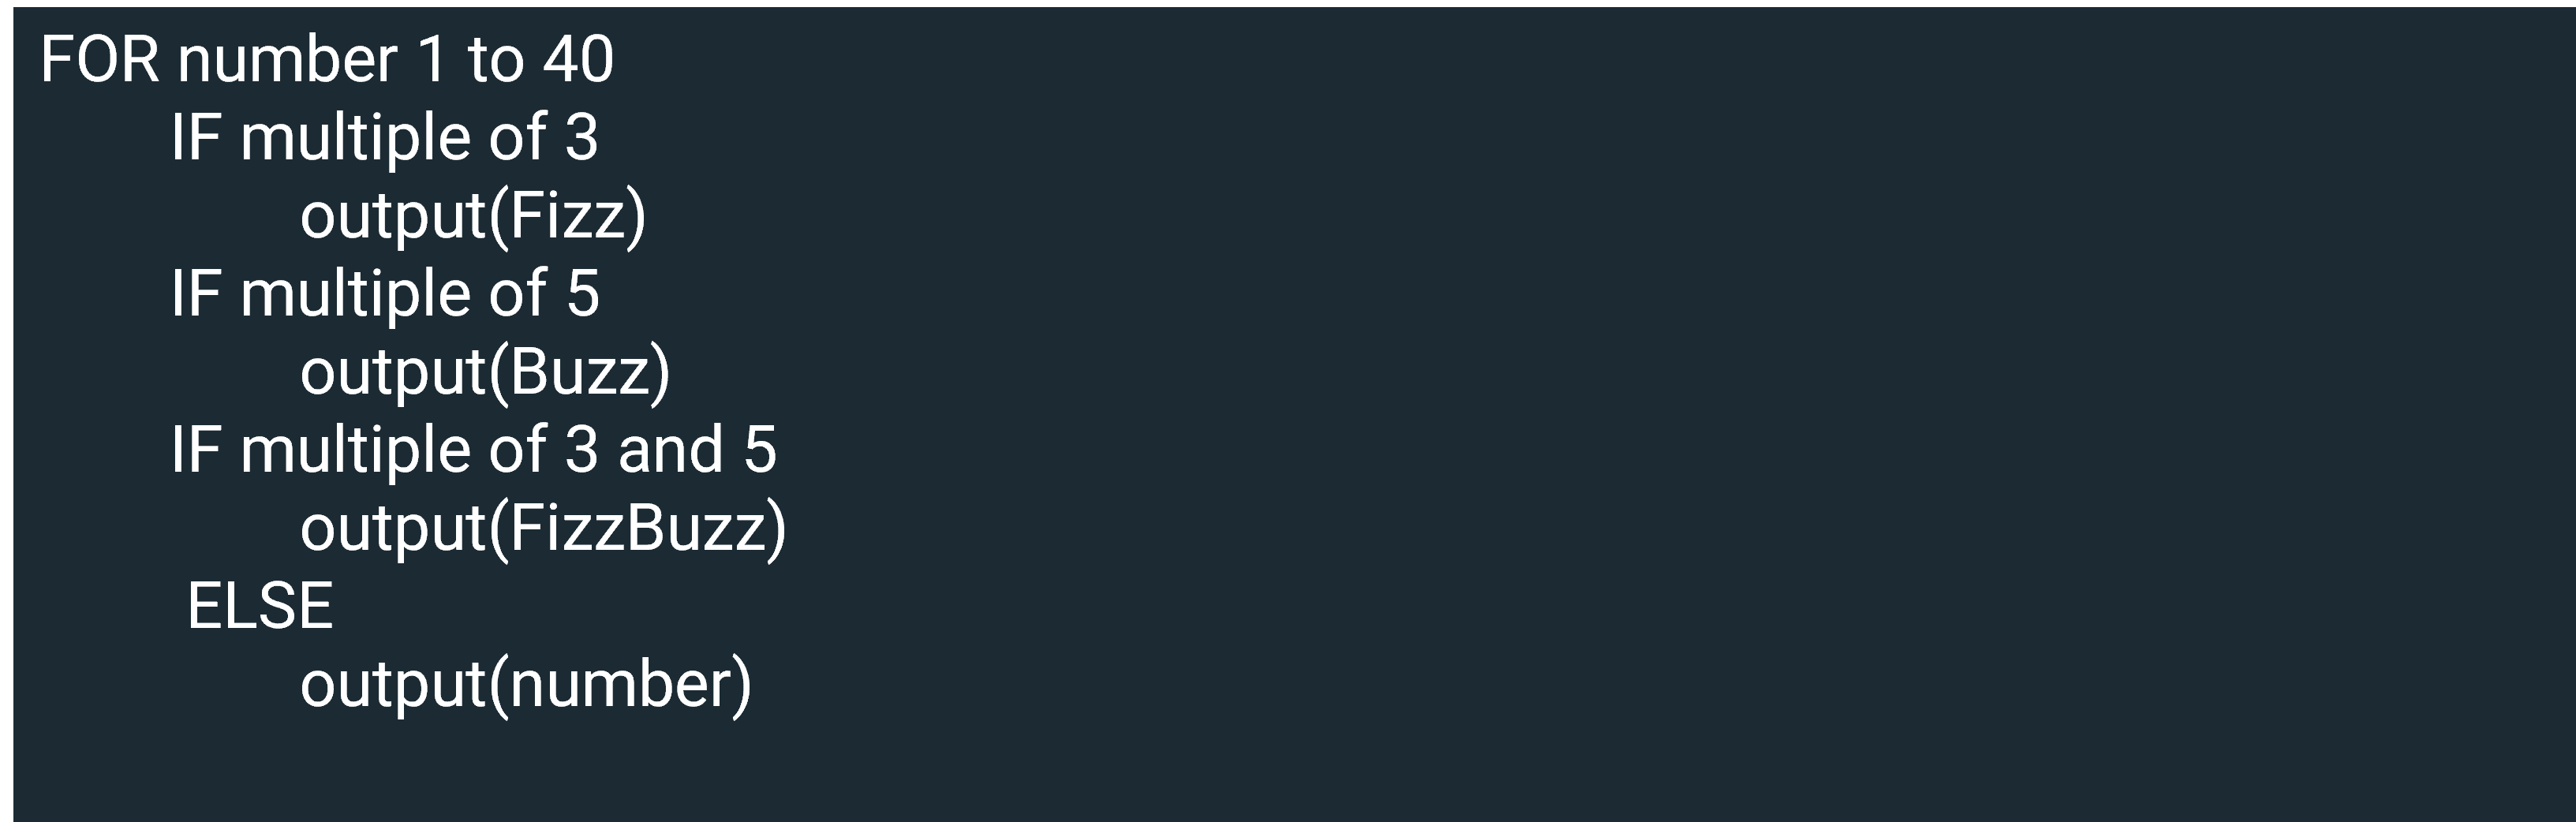
\includegraphics[width=0.8\textwidth]{./Picts/pseudocode1.png}
    \caption{}
\end{figure}

Kunci dari tugas ini adalah mengetahui cara mengatur pernyataan kondisional. Baris 1 menunjukkan bahwa akan ada iterasi. Dalam hal ini, indentasi menunjukkan bahwa delapan baris kode berikutnya merupakan bagian dari iterasi ini. Sebagai alternatif, blok berikut dapat ditambahkan:
\begin{figure}[H]
    \centering
    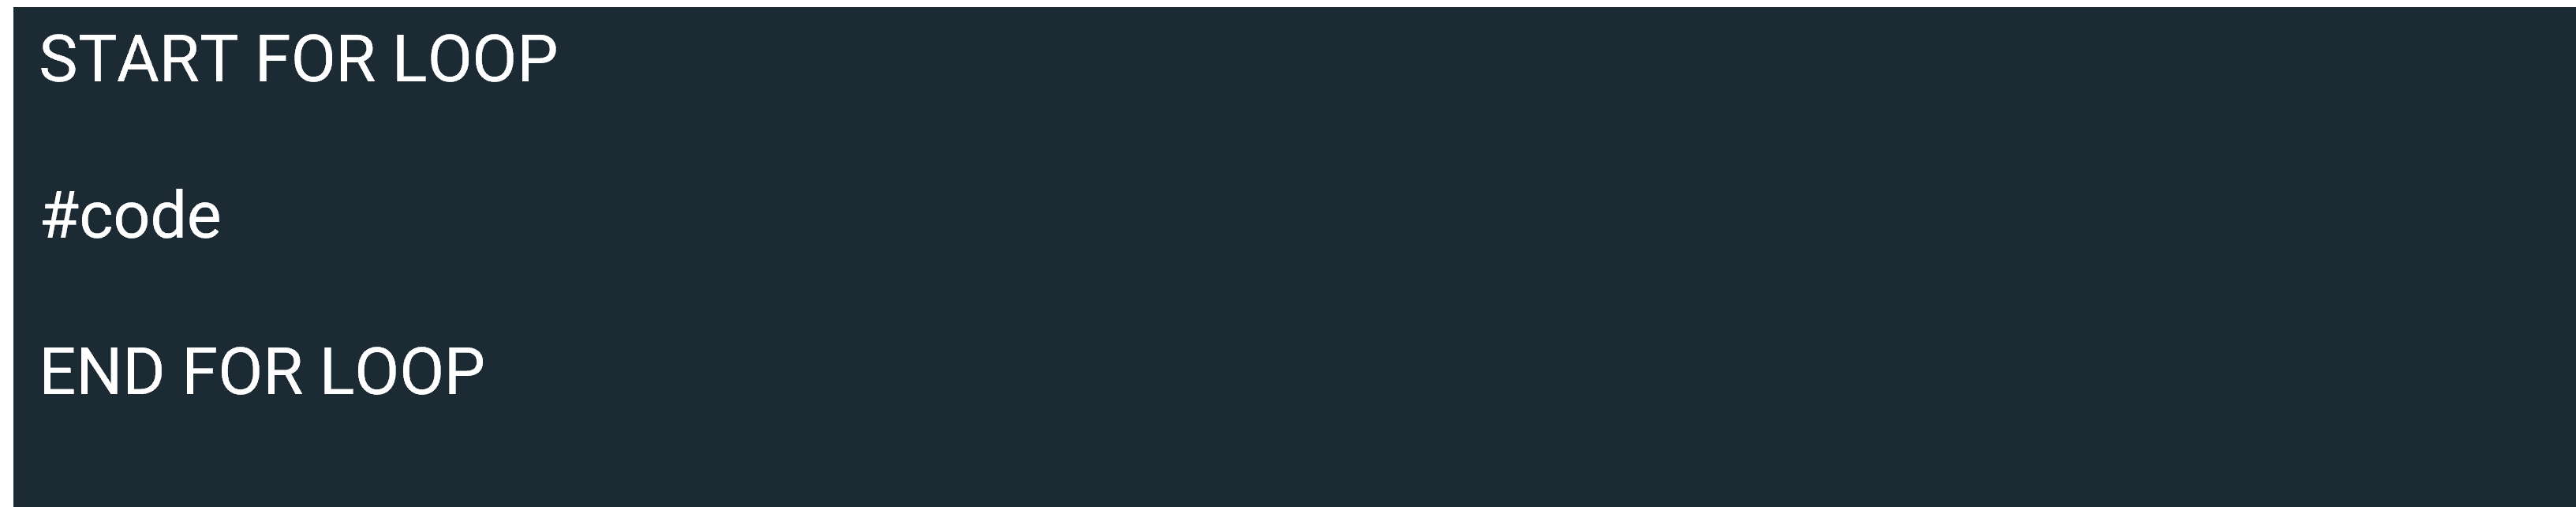
\includegraphics[width=0.8\textwidth]{./Picts/pseudocode2.png}
    \caption{}
\end{figure}

Jelas bahwa ada tiga pernyataan bersyarat dan kemudian klausa else yang mencakup semua kasus. Hasil kode dapat dibayangkan dengan melihat pseudocode. Pernyataan else akan berfungsi dengan baik, hanya mencetak angka yang bukan kelipatan 3 dan 5, tetapi ada masalah dengan cara kode menangani angka 15, yang mencetak contoh Fizz, Buzz, dan FizzBuzz.

\begin{figure}[H]
    \centering
    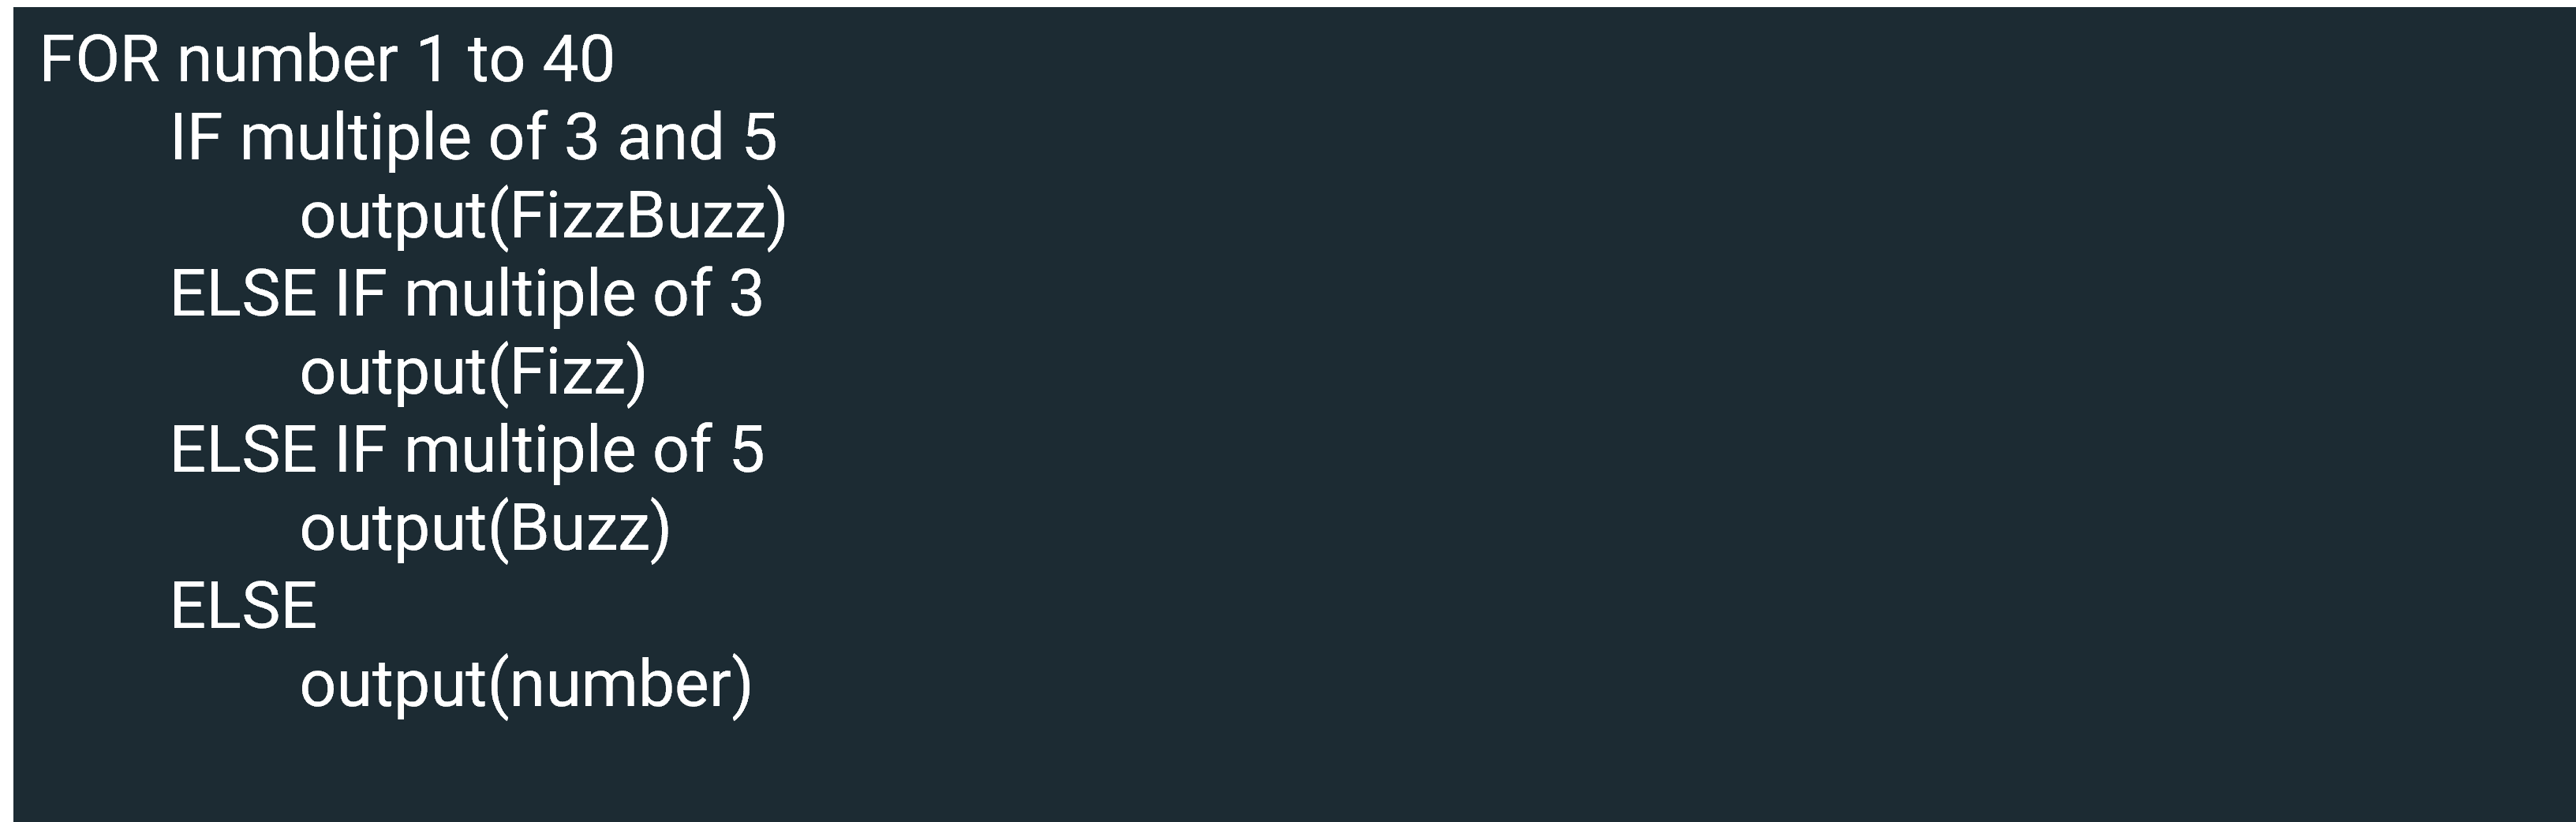
\includegraphics[width=0.8\textwidth]{./Picts/pseudocode3.png}
    \caption{}
\end{figure}

Menganalisis contoh pertama pertanyaan dalam bentuk pseudocode memungkinkan Anda untuk mengidentifikasi di mana masalah mungkin terjadi. Secara visual, jauh lebih mudah untuk melihat bagaimana pernyataan kondisional seharusnya disusun. Pertama, inti dari pertanyaan ini terletak pada urutan penempatan pernyataan kondisional dan penggunaan pernyataan kondisional eksklusif. Dalam contoh di atas, "else if" digunakan sebagai pengganti "if" saja. Kedua, urutan pernyataan memiliki dampak yang penting. Anda dapat mencoba output di atas dengan menjalankan kode yang terdapat di bawah ini.

\begin{lstlisting}[language=Python, caption={}, captionpos=b]
for number in range(1, 41):
    if number % 3 == 0 and number % 5 == 0:
        print("FizzBuzz")
    elif number % 3 == 0:
        print("Fizz")
    elif number % 5 == 0:
        print("buzz")
    else:
        print(number)
\end{lstlisting}

\subsection{Tips Interview}
\subsubsection{Persiapan}
Berikut adalah beberapa pertanyaan standar yang mungkin Anda temui dalam wawancara apa pun:
\begin{itemize}
    \item Ceritakan tentang diri Anda.
    \item Mengapa Anda merasa bahwa mereka seharusnya mempekerjakan Anda?
    \item Apa kelebihan utama Anda?
    \item Atau, apa kelemahan utama Anda?
    \item Berapa gaji yang Anda harapkan?
    \item Bagaimana pengalaman Anda sebelumnya membuat Anda cocok untuk peran ini?
    \item Apa yang dikatakan teman-teman Anda tentang Anda?
    \item Mengapa Anda ingin peran ini?
    \item Bagaimana Anda menangani konflik di masa lalu?
\end{itemize}

Mengetahui pertanyaan-pertanyaan ini akan datang memberikan keuntungan karena Anda dapat mempersiapkannya. Setelah membaca daftar ini, apakah Anda dapat menulis jawaban yang ringkas untuk masing-masing pertanyaan? Anda akan menemukan jawaban untuk banyak pertanyaan ini dalam resume Anda. Strategi yang baik adalah meninjau resume Anda sebelum wawancara untuk melihat aspek mana yang relevan dengan perusahaan dan posisi yang dilamar.

Jawaban tambahan yang layak dipersiapkan mungkin berkaitan dengan perusahaan itu sendiri. Di mana perusahaan tersebut bermarkas, dan apa yang mereka lakukan? Bagaimana pengalaman kerja Anda sebelumnya berkaitan dengan kebutuhan mereka saat ini? Teliti peran yang sama di perusahaan lain. Ketahui gaji pasar untuk posisi tersebut jika ditanya tentang besaran gaji. Pewawancara sudah tahu jawabannya, jadi mampu menjawab ini dengan baik menunjukkan kesiapan Anda. Mengetahui tentang perusahaan menunjukkan antusiasme untuk bekerja di sana. Akhirnya, pertimbangkan bahwa kelemahan juga dapat menjadi kekuatan. "Saya terlalu fokus pada detail" dapat merugikan jika ada tenggat waktu yang ketat; namun, hal itu menjadi kekuatan jika pekerjaan tersebut membutuhkan perhatian detail yang teliti.

\subsubsection{Soft skills}
Penyelesaian konflik merupakan keterampilan lunak yang sangat penting untuk dimiliki. Dalam kehidupan kerja Anda, Anda pasti akan menghadapi situasi di mana pendekatan atau tujuan Anda tidak sejalan dengan rekan kerja, atasan, atau pelanggan. Mengelola situasi-situasi ini membantu menciptakan lingkungan kerja yang harmonis. Sadari kapan Anda pernah berselisih dengan orang lain dan bagaimana Anda menyelesaikannya. Apakah pendekatan ini berhasil? Jika tidak, lakukan riset tentang cara menangani konflik di tempat kerja.

\subsubsection{Presentasi}
Seringkali dikatakan, "Berpakaianlah sesuai dengan pekerjaan yang kamu inginkan, bukan pekerjaan yang kamu miliki." Cara kamu tampil dapat secara tidak sadar menyampaikan banyak informasi tentang dirimu. Berpakaianlah rapi dan sopan. Rekan kerja masa depanmu mungkin ada di panel, dan kamu ingin membuat kesan yang baik. Pakaian yang kamu kenakan harus sesuai dengan peran yang kamu lamar. Kebanggaan terhadap penampilan dapat disamakan dengan kebanggaan terhadap peran yang diemban.

\subsubsection{Demeanor}
Tunjukkan kesiapan Anda untuk peran tersebut. Rekan kerja ingin melihat seseorang yang tertarik untuk berada di sana. Tetap tenang dan rileks saat menjawab pertanyaan. Tidak pernah disarankan untuk memotong pertanyaan. Dengarkan hingga pertanyaan selesai, lalu ambil napas. Pertanyaan tentang kompetensi memerlukan jawaban STAR (Situasi, Tugas, Tindakan, Hasil). Tunjukkan kebanggaan atas pengalaman kerja sebelumnya yang Anda miliki. Siapkan beberapa pertanyaan. Dalam wawancara, pewawancara selalu harus memberi Anda kesempatan untuk bertanya. Manfaatkan waktu ini untuk mengetahui apa yang dicari. Apa kondisi yang mungkin lebih menguntungkan bagi Anda? Apakah tujuan perusahaan sejalan dengan tujuan Anda, dan apakah Anda dapat mengkomunikasikannya?

Jadilah autentik dalam tindakan Anda. Lebih baik jujur dan terbuka saat melamar posisi. Berlebihan mungkin mengarah pada wawancara lanjutan, tetapi lebih baik mampu mengisi posisi apa pun yang Anda inginkan.

\subsubsection{Interview Virtual}
Banyak wawancara dilakukan secara virtual. Wawancara virtual menantang karena lebih sulit membaca bahasa tubuh melalui video. Karena kualitas suara, penting untuk tidak berbicara di atas orang lain. Pastikan semua perangkat teknologi Anda berfungsi dengan baik. Pastikan komputer Anda terhubung ke sumber daya dan memiliki headphone yang berfungsi jika terjadi masalah suara. Pastikan video Anda berfungsi dan kompatibel dengan platform. Terkadang, komputer perlu mengubah izin sebelum Anda dapat menggunakan kamera. Dan jangan lupa untuk menguji kecepatan koneksi.

Seperti halnya wawancara tatap muka, penampilan sangat penting. Luangkan waktu untuk memastikan Anda berpakaian sesuai. Meskipun Anda tidak berada di kantor, berpakaianlah seolah-olah Anda berada di sana. Seperti halnya wawancara tatap muka, perhatikan bahasa tubuh Anda. Duduklah dengan tegak dan tetap fokus. Meskipun Anda berada di rumah, tetaplah berperilaku sesuai etika kerja.

Temukan lokasi yang tenang dan bebas dari gangguan. Memiliki ruang kerja khusus dapat membantu. Hal ini diperlukan untuk memastikan bahwa selama wawancara, tidak ada tamu tak terduga yang melakukan pekerjaan rumah di latar belakang.

\subsection{Melakukan Tes terhadap Solusi}
Pengujian merupakan bagian penting dalam pengembangan perangkat lunak. Idealnya, cakupan pengujian Anda harus komprehensif; namun, selalu ada faktor eksternal yang dapat memengaruhi hasil ideal ini. Secara historis, pengujian sering dilakukan di akhir proses, sehingga jika tenggat waktu produksi mendekat, pengujian sering menjadi hal pertama yang dikurangi. Test-Driven Development (TDD) adalah pendekatan yang dikembangkan untuk menghindari hasil tersebut. Pembahasan tentang pengujian ini akan berfokus pada dua contoh, yaitu wawancara coding dan tugas yang dibawa pulang.

\subsubsection{Tugas Take-home}
Jika Anda diizinkan untuk membawa kode pulang, Anda mungkin memiliki waktu untuk mengimplementasikan tes yang lebih komprehensif.

Ada banyak jenis tes yang dapat Anda pilih untuk dijalankan. Misalnya:
\begin{itemize}
    \item Tes integrasi: Tes ini menguji bagaimana berbagai komponen aplikasi berinteraksi satu sama lain. Tes integrasi tidak akan mendalam karena ketergantungan eksternal akan disimulasikan daripada menggunakan instance aktual. Selain itu, unit testing untuk menilai baris kode yang lebih sepsifik, sementara uji integrasi mengambil pendekatan yang lebih global.
    \item Uji fungsional: Ini adalah uji otomatis yang membuktikan bahwa sistem beroperasi sesuai harapan. Uji ini berfokus pada kemampuan sistem.
    \item Uji regresi: Ini untuk memastikan bahwa perubahan tidak menyebabkan kesalahan pada kode yang sudah ada. Uji ini memastikan bahwa ketika perubahan sistem dilakukan, hal itu tidak memengaruhi operasinya.
\end{itemize}

Tingkat pengujian yang Anda terapkan selalu bergantung pada waktu yang tersedia. Bagian penting dari proses ini adalah mengembangkan aplikasi yang berfungsi. Pengujian menunjukkan ketelitian Anda dan memastikan bahwa aplikasi tersebut akan berfungsi dengan baik. Sejauh mana Anda dapat menerapkan strategi-strategi ini mungkin terbatas tergantung pada waktu yang Anda miliki.

\subsubsection{Interview Coding}
Unit testing adalah pendekatan yang memastikan kode Anda berfungsi sesuai yang diharapkan. Meskipun banyak pengujian ditulis sebelum kode masuk ke produksi, Anda tidak akan memiliki kesempatan untuk menulis semua pengujian ini saat mengikuti wawancara coding. Pengujian unit adalah pendekatan yang dapat dikelola dan dapat diintegrasikan ke dalam solusi Anda, menunjukkan perhatian Anda terhadap detail. Hal ini akan menunjukkan praktik pengujian kode yang baik.

Pengujian unit kurang fokus pada operasi keseluruhan aplikasi. Sebaliknya, pengujian ini memastikan bahwa setiap komponen individu berfungsi sesuai yang diharapkan.

\paragraph{Pertimbangan ketika menulis test}

\begin{itemize}
    \item Keterbacaan: Buatlah tes yang mudah dibaca oleh pengembang lain. Kebiasaan ini harus diinternalisasi terlepas dari apakah Anda bekerja dalam tim. Tes dengan tujuan yang jelas dapat mengidentifikasi masalah jika terjadi. Mereka juga menunjukkan apa yang seharusnya dicapai oleh bagian kode tertentu. Hal ini juga meningkatkan keterpeliharaan kode.
    \item Hasil yang jelas: Tes Anda sebaiknya, sejauh mungkin, bersifat deterministik. Artinya, hasilnya harus selalu sama terlepas dari kondisi yang ada. Tes deterministik akan selalu gagal jika kode bermasalah ditulis. Tes yang bergantung pada kombinasi kondisi yang berbeda dapat menyulitkan proses debugging.
    \item Otomatisasi: Tes harus selalu memiliki potensi untuk diotomatisasi sehingga dapat dijalankan dengan cepat setiap kali perubahan dilakukan pada kode. Ini merupakan landasan utama CI/CD (Continuous Integration/Continuous Development).
\end{itemize}

\paragraph{Menggunakan unit test kedalam praktek}
Panduan solusi utama menjelaskan langkah-langkah yang diperlukan untuk membuat permainan menebak angka. Di bawah ini adalah tangkapan layar dari pseudocode yang digunakan untuk mengembangkan solusi yang layak.
\begin{figure}[H]
    \centering
    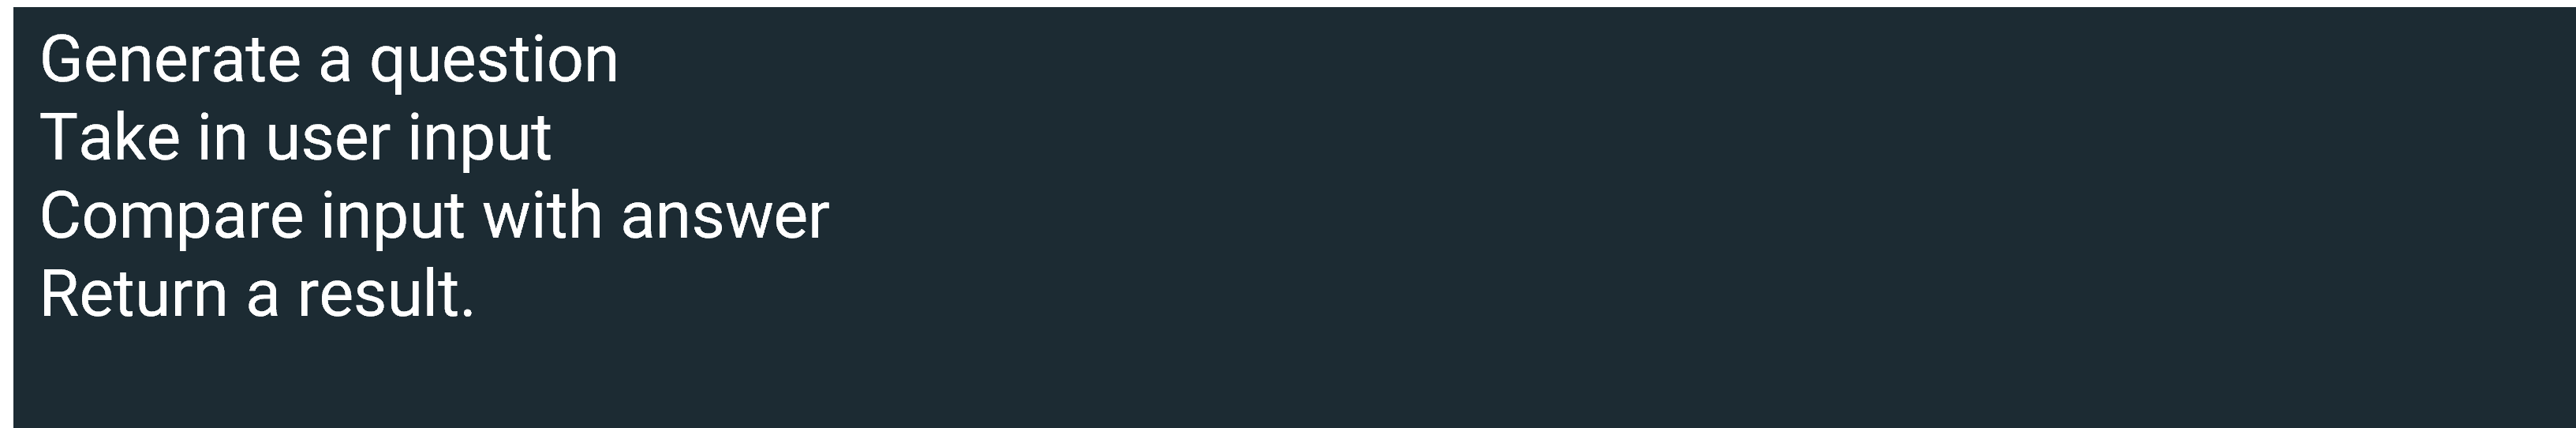
\includegraphics[width=0.8\textwidth]{./Picts/unittes1.png}
    \caption{}
\end{figure}

Mengambil contoh ini, bayangkan bahwa hanya tersisa beberapa menit dari waktu yang dialokasikan, apa yang akan Anda fokuskan? Uji unit paling dasar yang dapat ditulis adalah kasus asersi, yang memastikan bahwa apa yang diberikan sesuai dengan yang diharapkan. Perpustakaan untuk ini tersedia di sebagian besar bahasa pemrograman.
\begin{figure}[H]
    \centering
    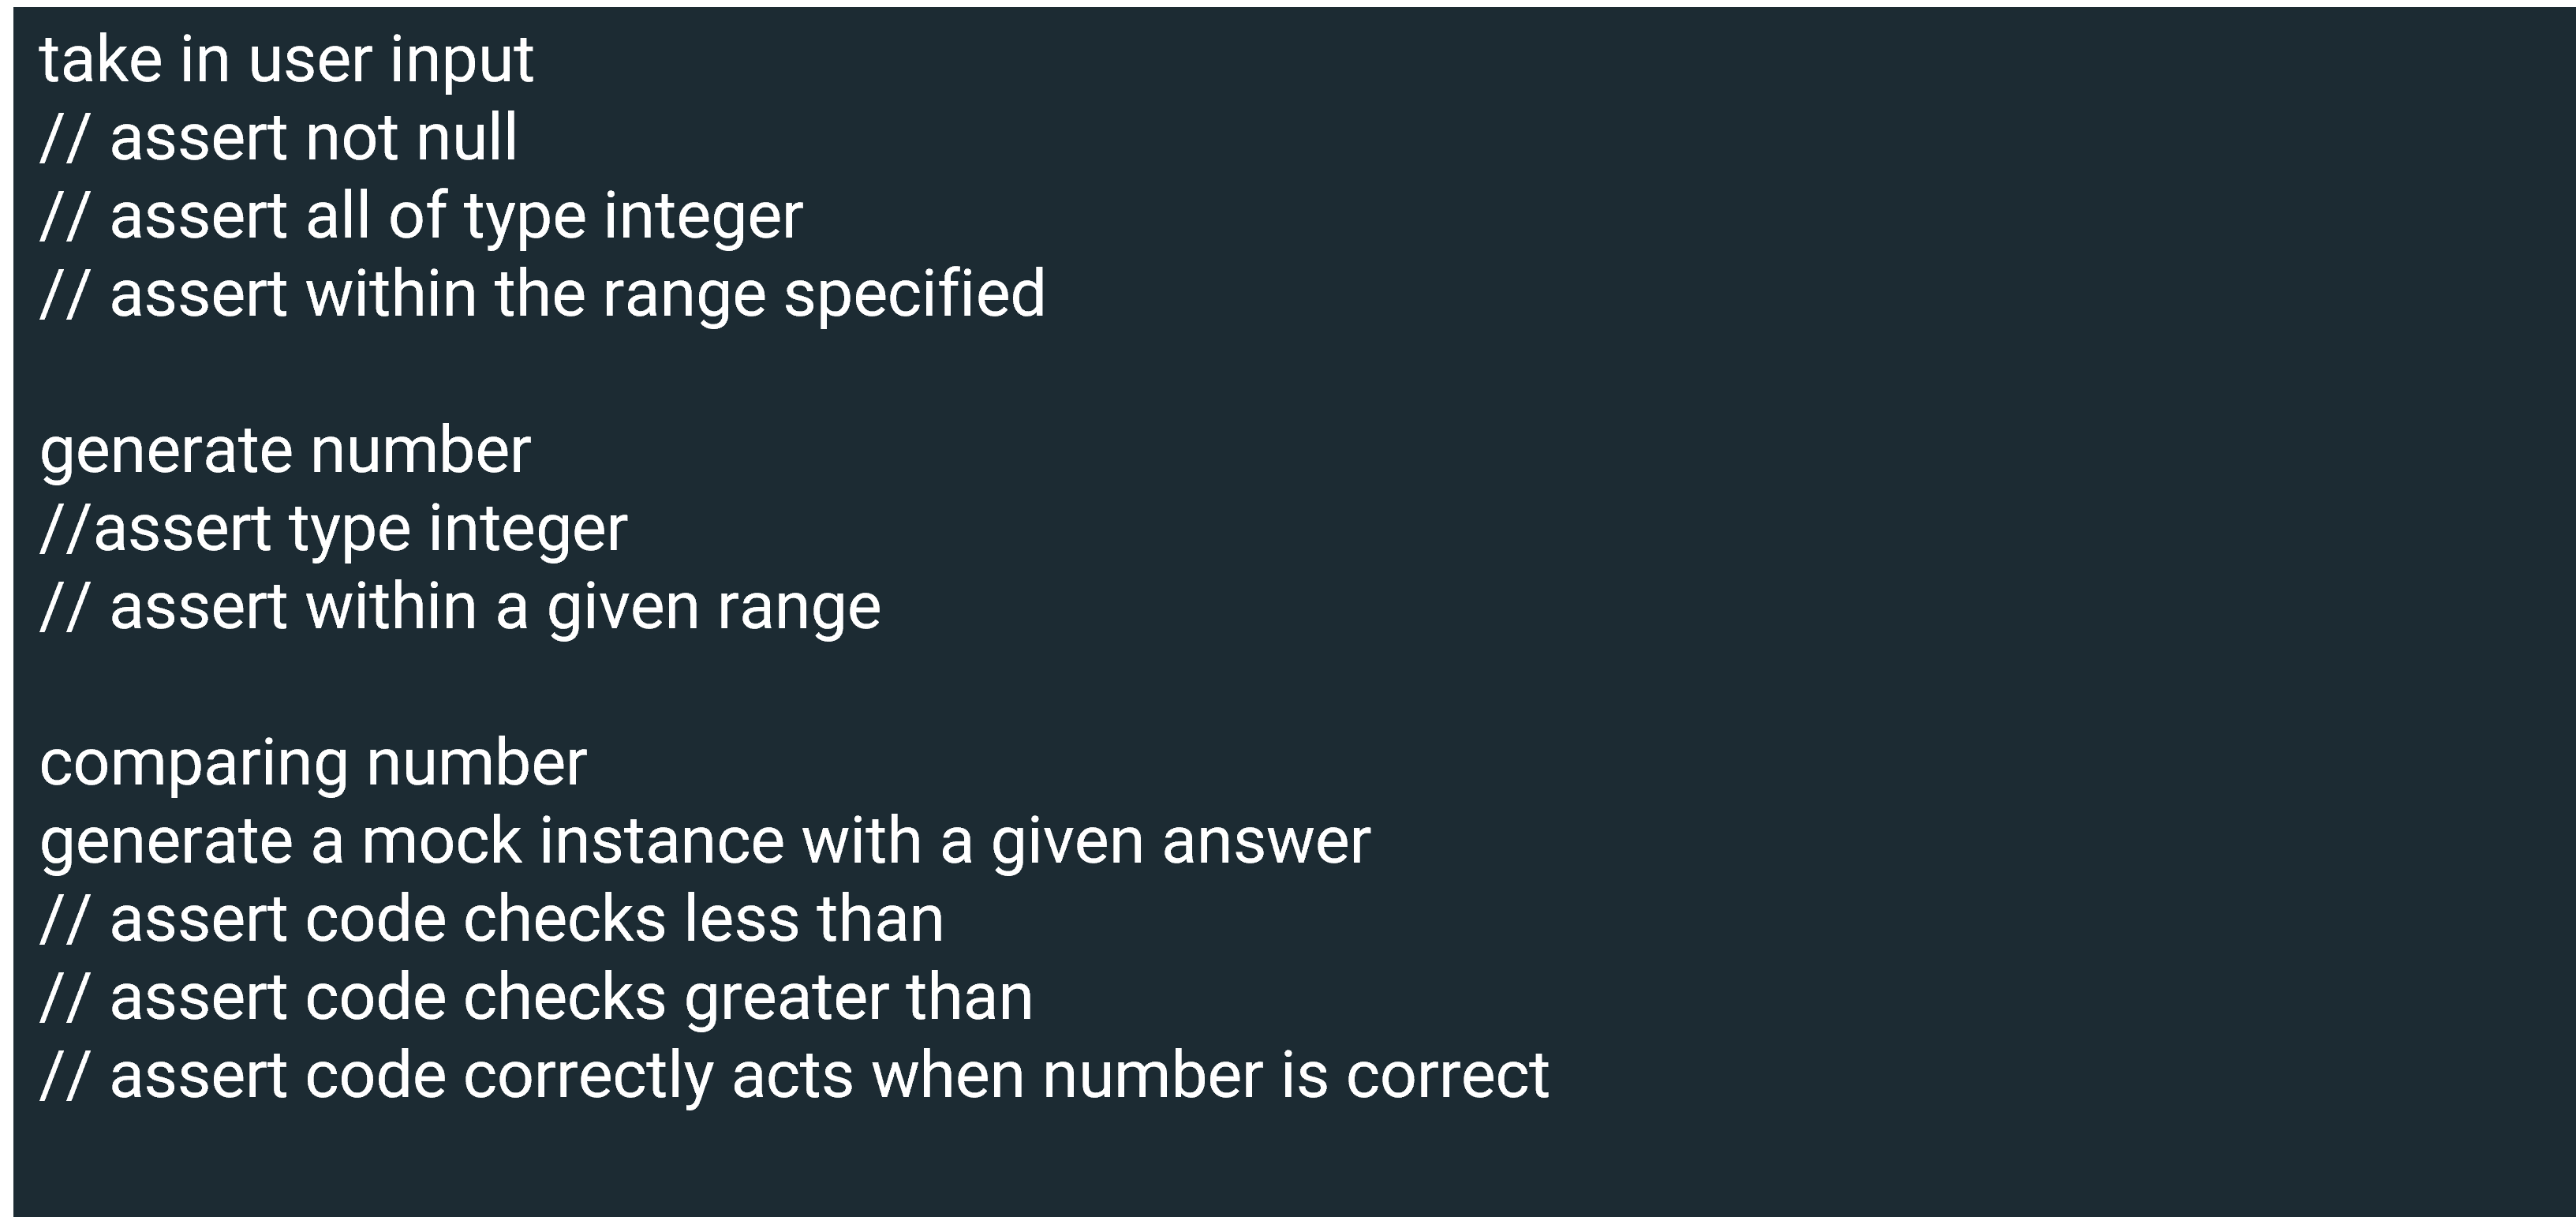
\includegraphics[width=0.8\textwidth]{./Picts/unittes2.png}
    \caption{}
\end{figure}

Langkah pertama mungkin adalah menulis kasus uji untuk menentukan apakah masukan pengguna valid. Baris 2–4 menjelaskan beberapa tes yang dapat diterapkan untuk memvalidasi masukan pengguna, memastikan bahwa sesuatu telah dimasukkan sebelum pengguna menekan tombol return. Anda harus memastikan bahwa masukan tersebut memiliki tipe yang benar dan tidak akan menyebabkan program crash. Selain itu, pastikan masukan tersebut berada dalam batas yang ditentukan. Selanjutnya, pertimbangkan untuk memeriksa angka acak yang dihasilkan. Apakah jenisnya benar dan apakah berada dalam parameter yang dapat diterima? Akhirnya, akan membantu jika Anda mempertimbangkan untuk menyertakan pemeriksaan yang memastikan hasil yang benar saat pernyataan kondisional diaktifkan.

Proses penulisan uji unit telah distandardisasi. Disarankan untuk berlatih mengimplementasikannya saat Anda menulis kode. Hal ini akan membantu Anda cepat familiar dengan proses tersebut dan dapat menyoroti kesadaran Anda dalam lingkungan di mana Anda menguji kode Anda.

\subsection{Angka Biner}
\begin{itemize}
    \item Binary Numbers: Sistem angka yang hanya menggunakan dua digit, yaitu 0 dan 1. Komputer menggunakan angka biner untuk menyimpan dan memproses informasi.
    \item Positional Notation: Metode di mana posisi angka menentukan nilai. Dalam sistem biner, setiap posisi mewakili pangkat dua (\(2^n\)).
\end{itemize}

\subsection{Representasi dan Penyimpanan}
\begin{itemize}
    \item Byte: Unit penyimpanan data yang terdiri dari 8 bits. Setiap bit dapat bernilai 0 atau 1.
    \item Exponentiation: Proses menghitung pangkat suatu angka. Misalnya, \(2^3 = 2 * 2 * 2 = 8\). Ini digunakan untuk menentukan jumlah kombinasi yang dapat diwakili oleh byte.
\end{itemize}

\subsection{Contoh Aplikasi Biner dalam Komputer}
\begin{itemize}
    \item Boolean Values: Nilai yang hanya dapat bernilai true (1) atau false (0). Digunakan dalam logika komputer.
    \item ASCII (American Standard Code for Information Interchange): Kode yang memetakan angka biner ke karakter. Setiap karakter memiliki representasi biner yang unik.
\end{itemize}

\subsection{Contoh Hitung Kombinasi}
\begin{itemize}
    \item Lock Example: Jika sebuah kunci memiliki 4 digit biner, jumlah kombinasi yang mungkin adalah \(2^4 = 16\). Jika 5 digit, maka \(2^5 = 32\).
    \item Total Representations in a Byte: Dengan 8 bits, jumlah kombinasi yang dapat diwakili adalah \(2^8 = 256\).
\end{itemize}

\subsection{Bekerja dengan Binary}
Anda mungkin berpikir bahwa menggunakan hanya dua masukan terlalu membatasi. Faktanya, hal ini sangat fleksibel dan menawarkan berbagai pilihan yang luas ketika digabungkan dengan aljabar Boolean dan sirkuit.

\subsubsection{Logika Boolean}
Fungsi Boolean memetakan dua masukan ke sebuah nilai. Masukan-masukan ini dibatasi pada dua keadaan. Keadaan-keadaan ini dapat diartikan sebagai: on/off, true/false, atau 1/0. Untuk mendefinisikan fungsi Boolean, Anda hanya perlu menentukan bagaimana keluaran ditentukan untuk semua masukan yang mungkin. Berikut adalah contoh 4 fungsi:
\begin{figure}[H]
    \centering
    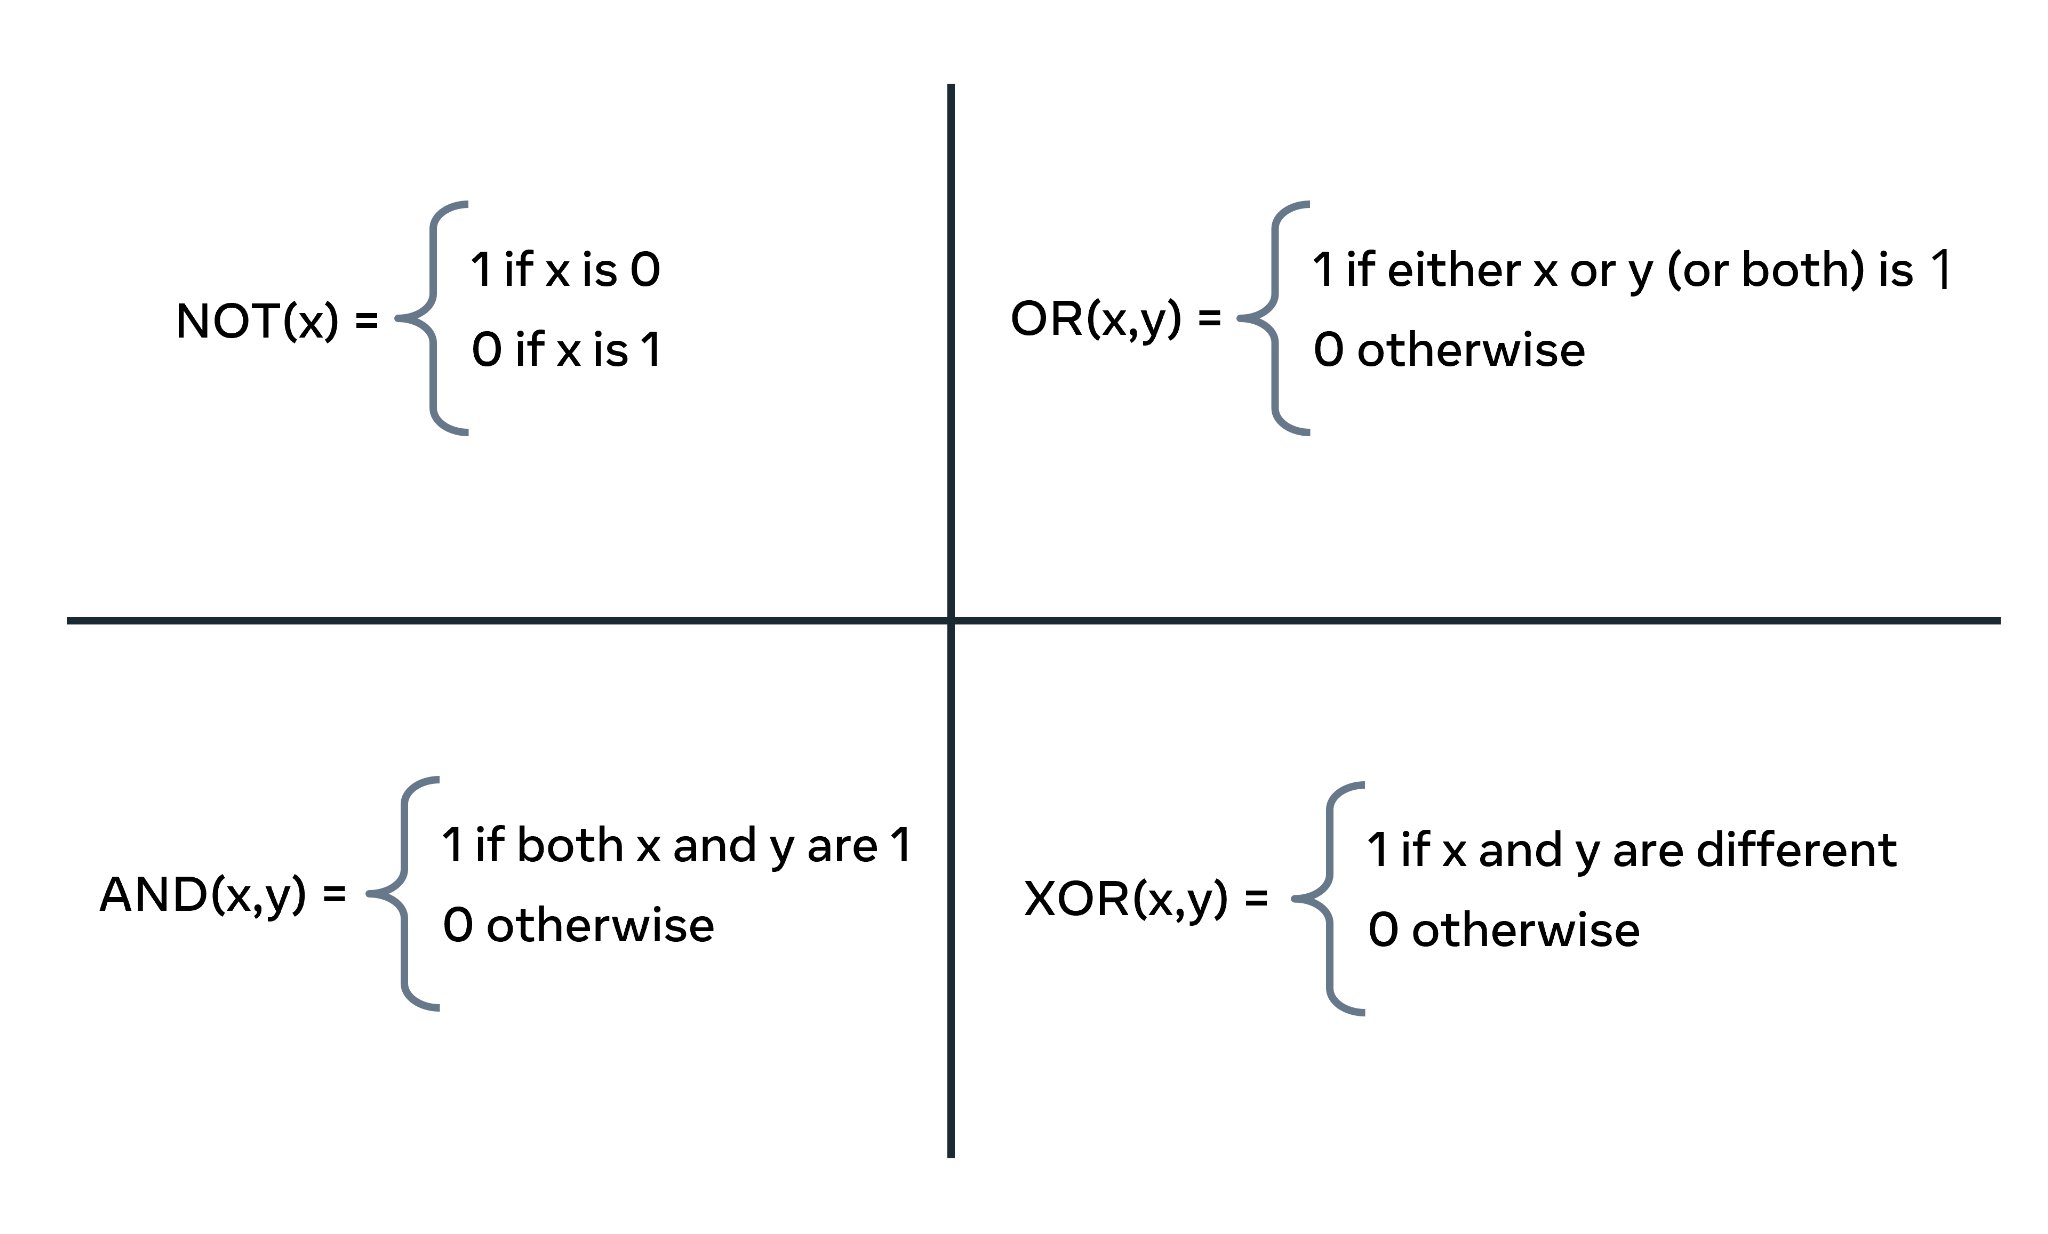
\includegraphics[width=0.8\textwidth]{./Picts/bool_logic.png}
    \caption{}
\end{figure}

\verb|NOT| menerima satu nilai x dan mengembalikan hasilnya sebagai 0 atau 1. \verb|OR| menerima dua argumen (x, y) untuk menghasilkan keluaran 1. Hanya salah satu dari nilai x atau y yang harus bernilai 1, atau keduanya sekaligus. Jika kedua nilai tersebut 0 secara bersamaan, keluaran adalah 0. \verb|AND| memerlukan kedua masukan untuk bernilai 1 sebelum dapat menghasilkan 1. Akhirnya, \verb|XOR| akan menerima dua nilai apa pun dan menentukan apakah keduanya berbeda; jika ya, outputnya adalah 1. Dalam semua kasus lain, hasilnya adalah 0.

\begin{figure}[H]
    \centering
    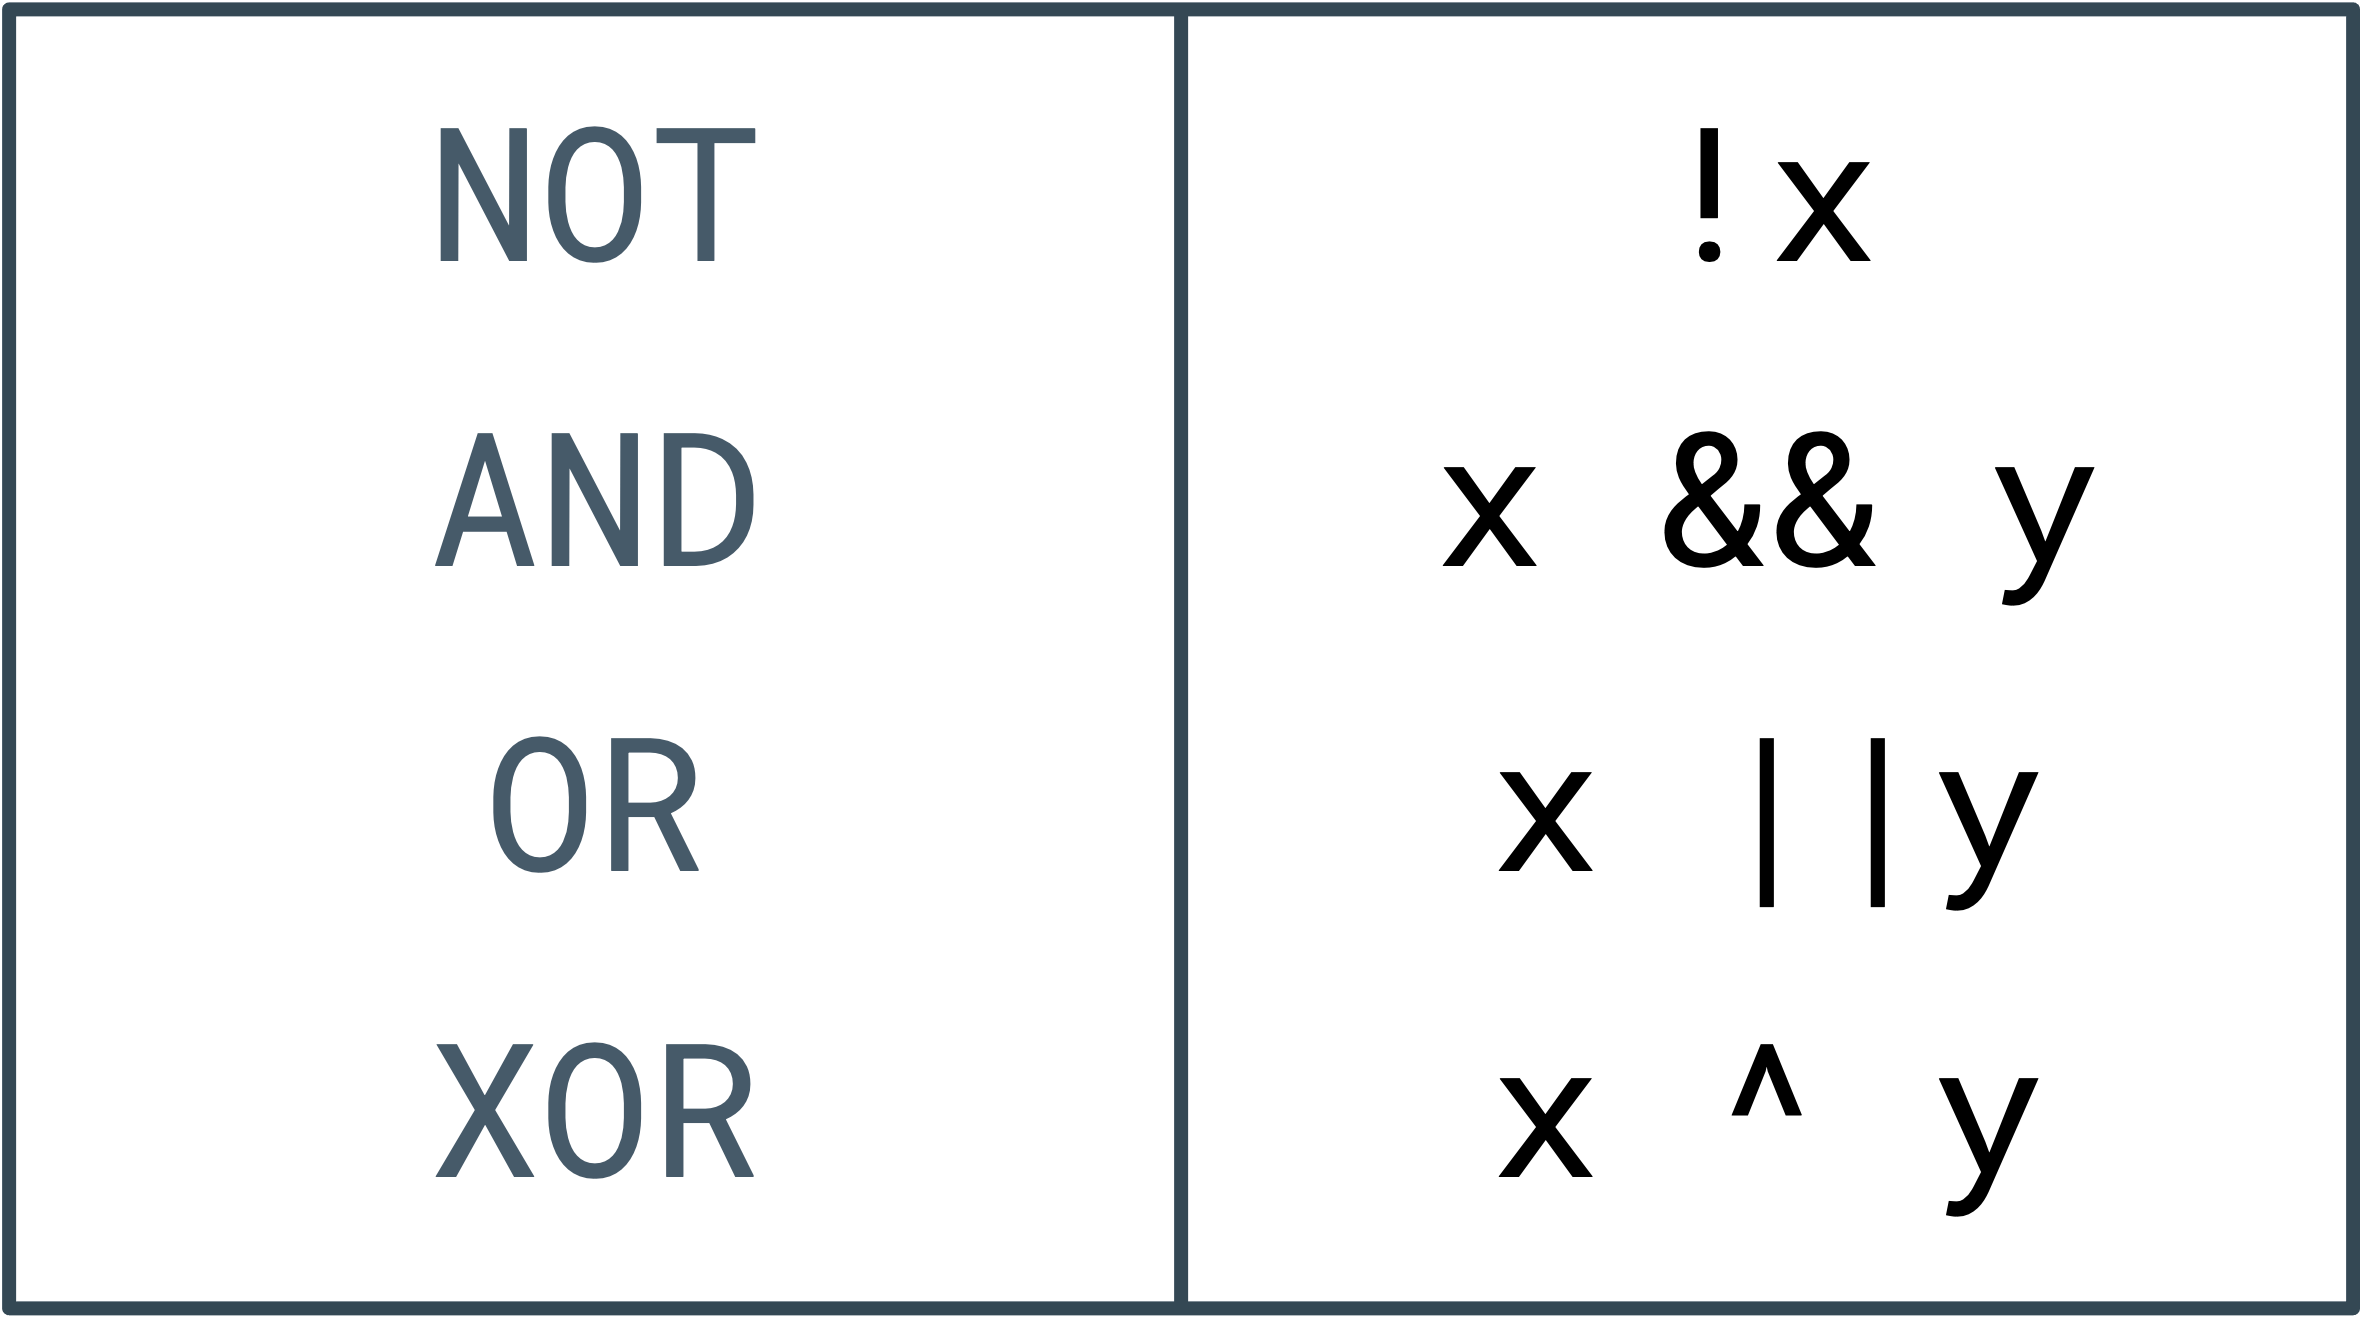
\includegraphics[width=0.8\textwidth]{./Picts/bool_logic2.png}
    \caption{}
\end{figure}

Konsep yang sama dapat diwakili secara komputasional. Dalam tabel ini, ekspresi Boolean berada di sebelah kiri, dan simbol komputasionalnya berada di sebelah kanan. Umumnya, ekspresi ini digabungkan dengan pernyataan kondisional atau iterator. Oleh karena itu, Anda dapat mengharapkan kode yang mirip dengan potongan kode berikut:

\begin{figure}[H]
    \centering
    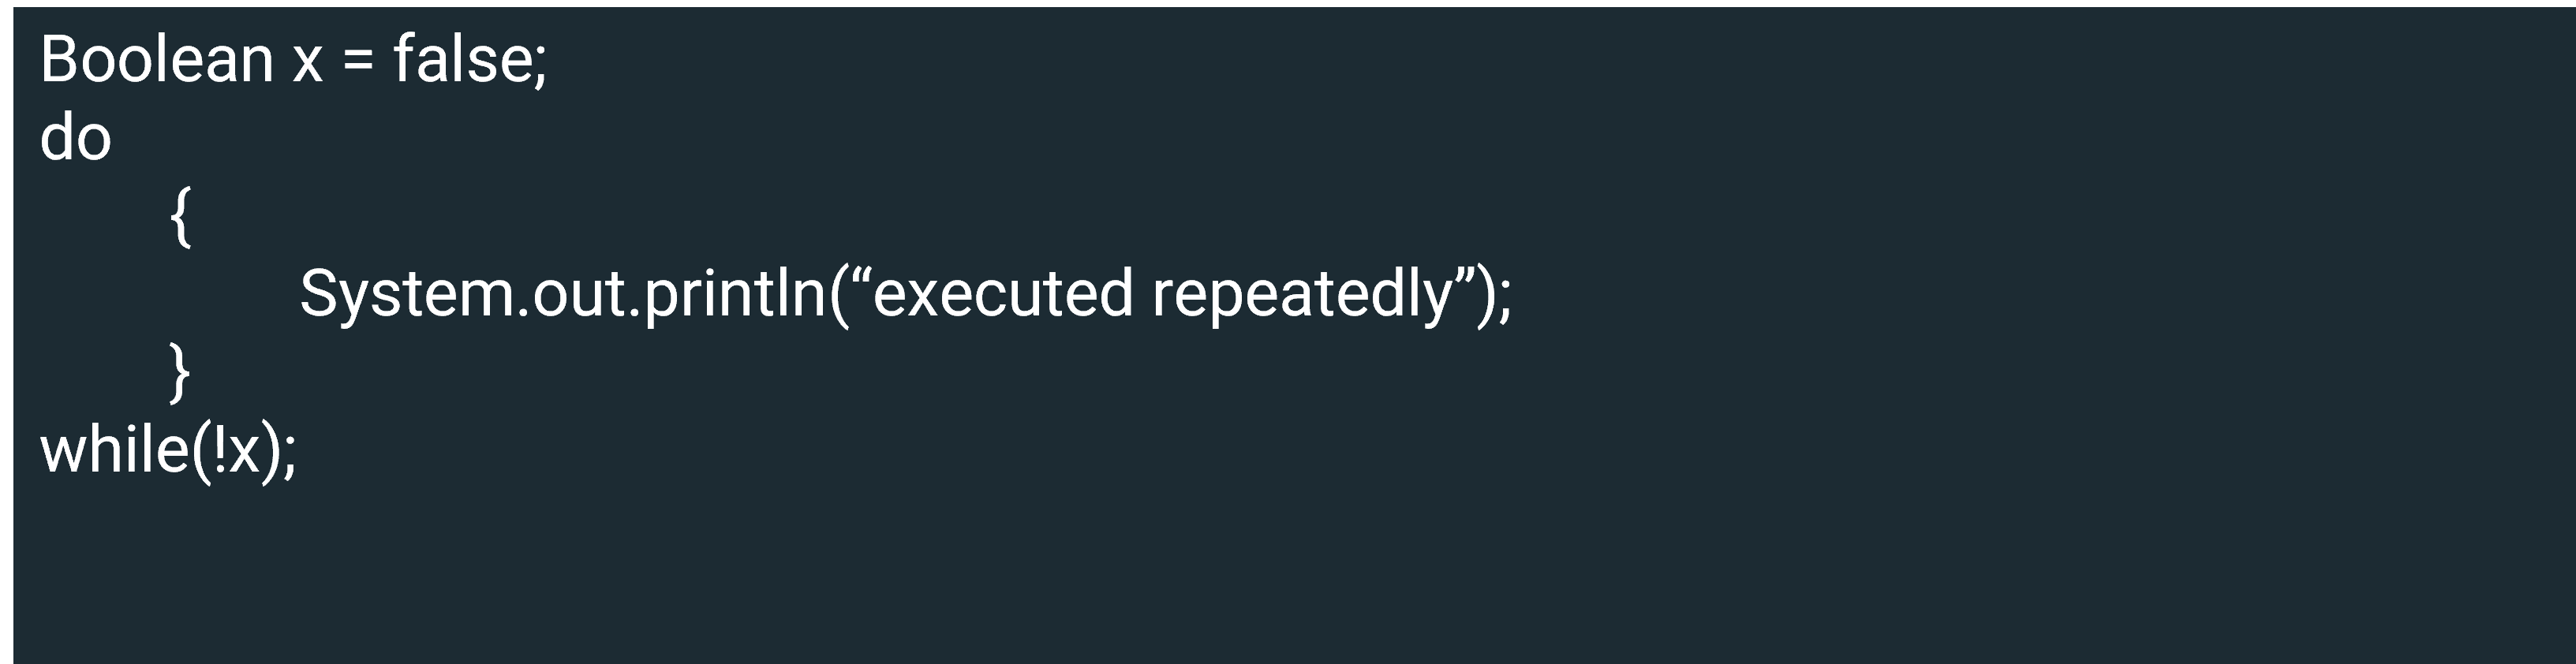
\includegraphics[width=0.8\textwidth]{./Picts/bool_logic3.png}
    \caption{}
\end{figure}

Dalam kode di atas, sebuah variabel Boolean telah disetel ke false. Sebuah loop do/while kemudian terus-menerus menjalankan kode yang terdapat di dalam blok do hingga nilai x berubah menjadi true. Secara umum, Anda akan mencari hasil tertentu, dan penggunaan logika Boolean memungkinkan Anda untuk terus mencari hingga hasilnya menjadi true. Perhatikan bagaimana fungsi NOT diterapkan dalam loop while untuk menguji apakah iterasi lain harus dilakukan.

\subsubsection{Tabel Kebenaran}
Mengingat jumlah keluaran yang terbatas dari fungsi Boolean, dimungkinkan untuk menggambarkan semua permutasi ke dalam tabel.

\begin{figure}[H]
    \centering
    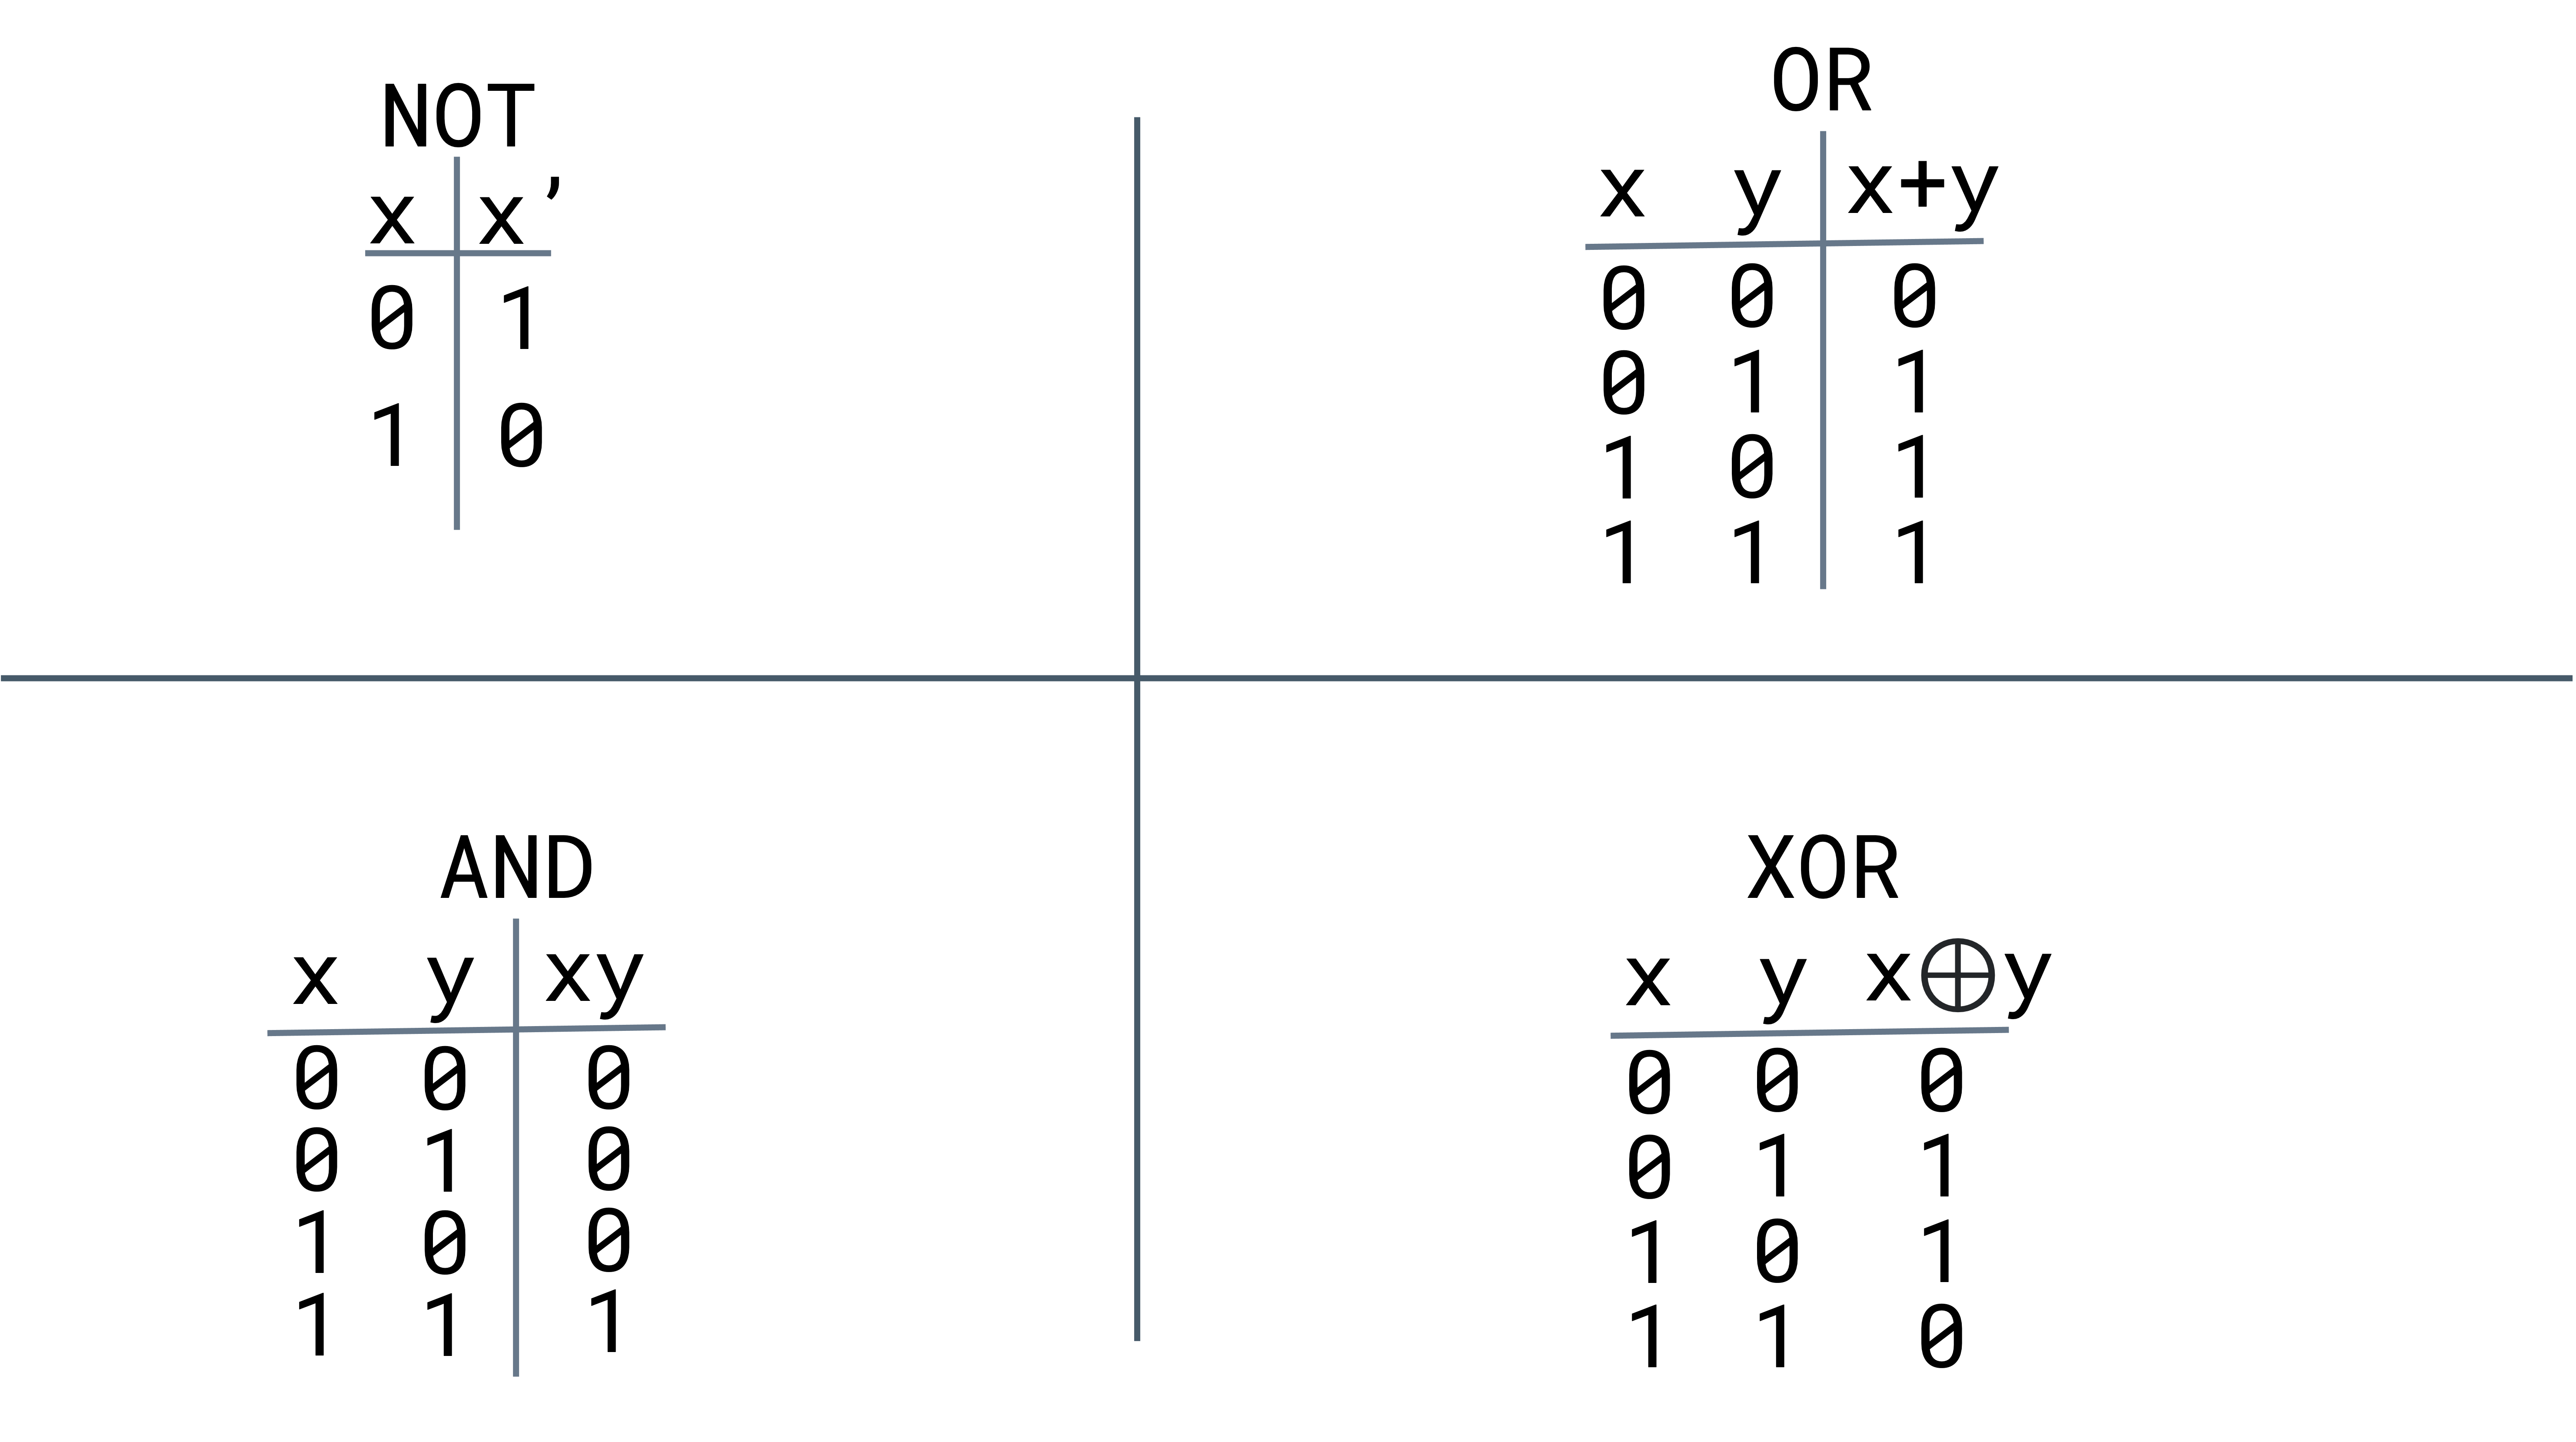
\includegraphics[width=0.8\textwidth]{./Picts/tabel_kebenaran.png}
    \caption{}
\end{figure}

Gambar ini menunjukkan semua kombinasi untuk setiap fungsi Boolean. Kolom X dan Y menunjukkan apakah menerima nilai 0 atau 1, sedangkan kolom XY menunjukkan hasil akhir. Fungsi NOT hanya memiliki satu keluaran dan satu masukan, sehingga tabelnya hanya berukuran 2 x 2. Dibandingkan dengan itu, ketiga contoh lainnya masing-masing menerima dua masukan dan menghasilkan satu hasil.

\subsubsection{Gerbang-gerbang}
Bahan dasar utama untuk sirkuit logika digital adalah gerbang. Fungsi logika kemudian diimplementasikan melalui interkoneksinya. Gerbang adalah sirkuit elektronik yang menghasilkan keluaran Boolean dari masukan-masukannya.

\begin{figure}[H]
    \centering
    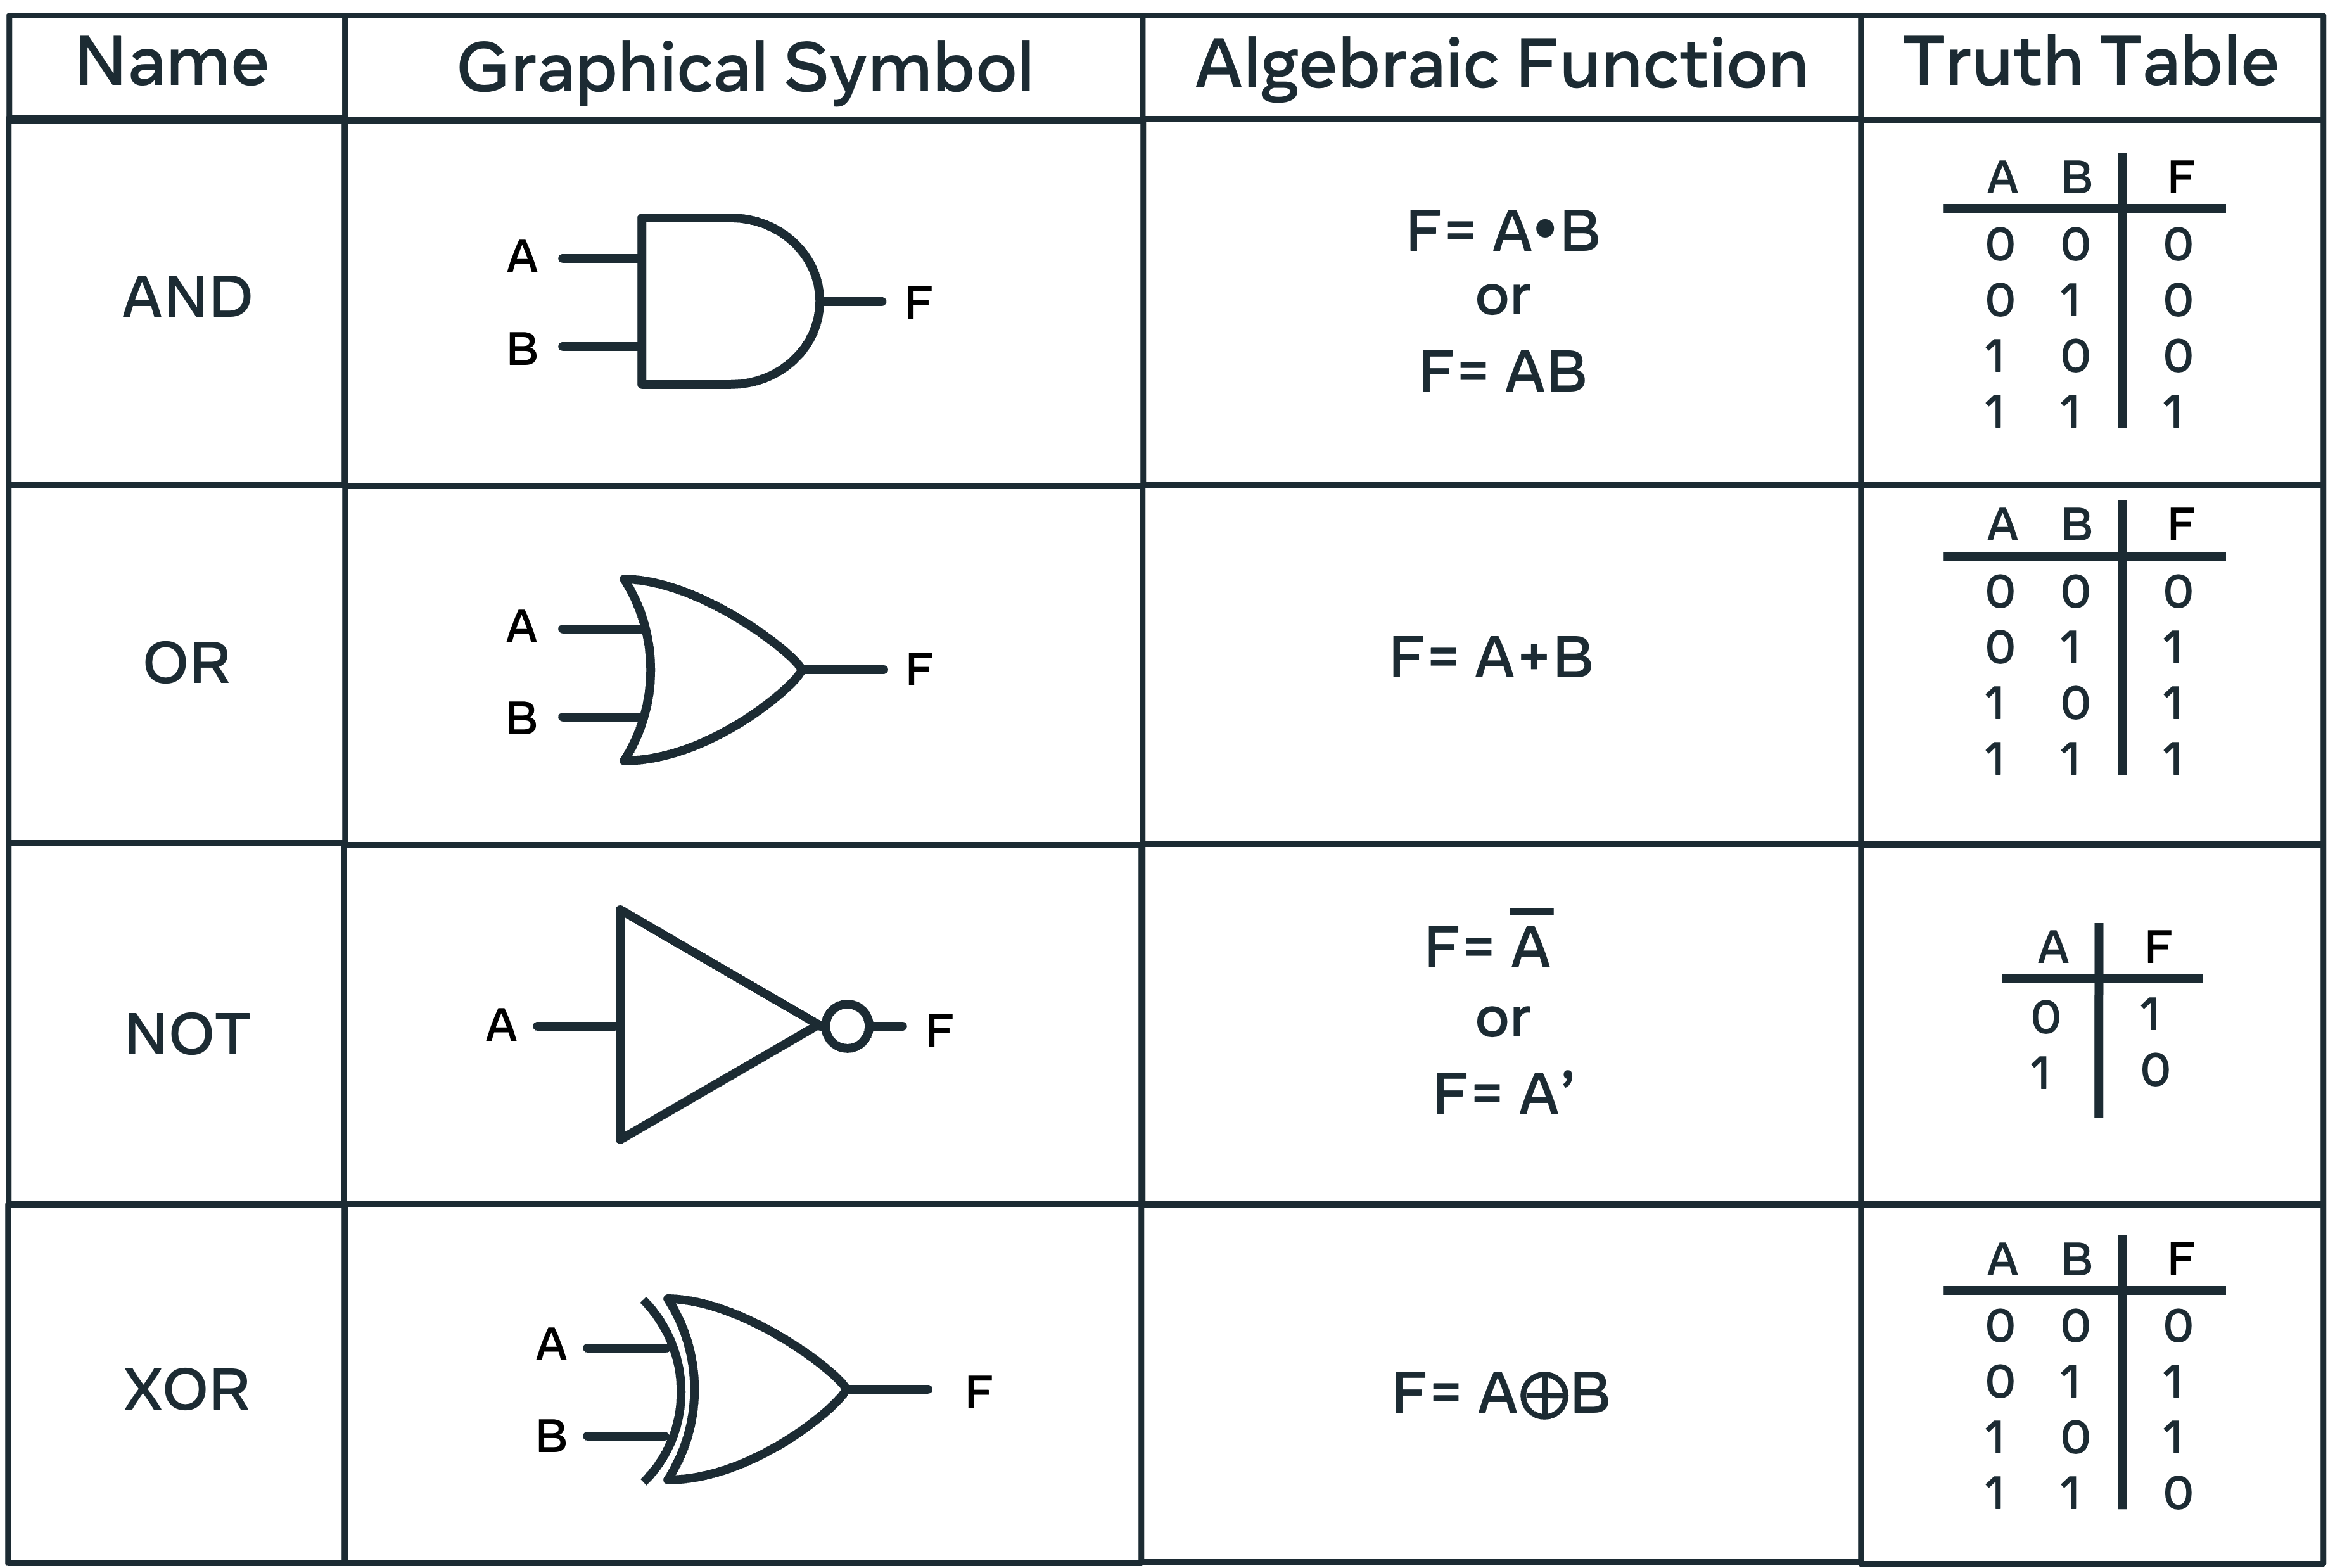
\includegraphics[width=0.8\textwidth]{./Picts/gerbang.png}
    \caption{}
\end{figure}

Pada gambar di atas, empat fungsi Boolean dasar ditampilkan. Simbol Grafis menunjukkan cara gerbang-gerbang ini digambarkan pada diagram. Anda sering akan menemui diagram sirkuit yang berisi serangkaian gerbang yang saling terhubung. Fungsi Aljabar menunjukkan cara gerbang-gerbang ini dijelaskan ketika ditulis dalam bentuk rumus.

Akhirnya, tabel kebenaran menggambarkan hasil dari masukan tertentu ke gerbang. Pada tingkat dasar, setiap masukan yang dilambangkan dengan A dan B mewakili arus yang dapat mengalir melalui sirkuit. Masukan-masukan ini dapat terhubung ke saklar atau tombol yang dapat diaktifkan untuk mengirimkan nilai 0 atau 1. Ekspresi logika Boolean ini terbentuk ketika gerbang sirkuit digabungkan untuk membentuk sirkuit yang kompleks. Keluaran akhir Q ditentukan berdasarkan operasi yang dilakukan pada masukan A, B, dan C.

\begin{figure}[H]
    \centering
    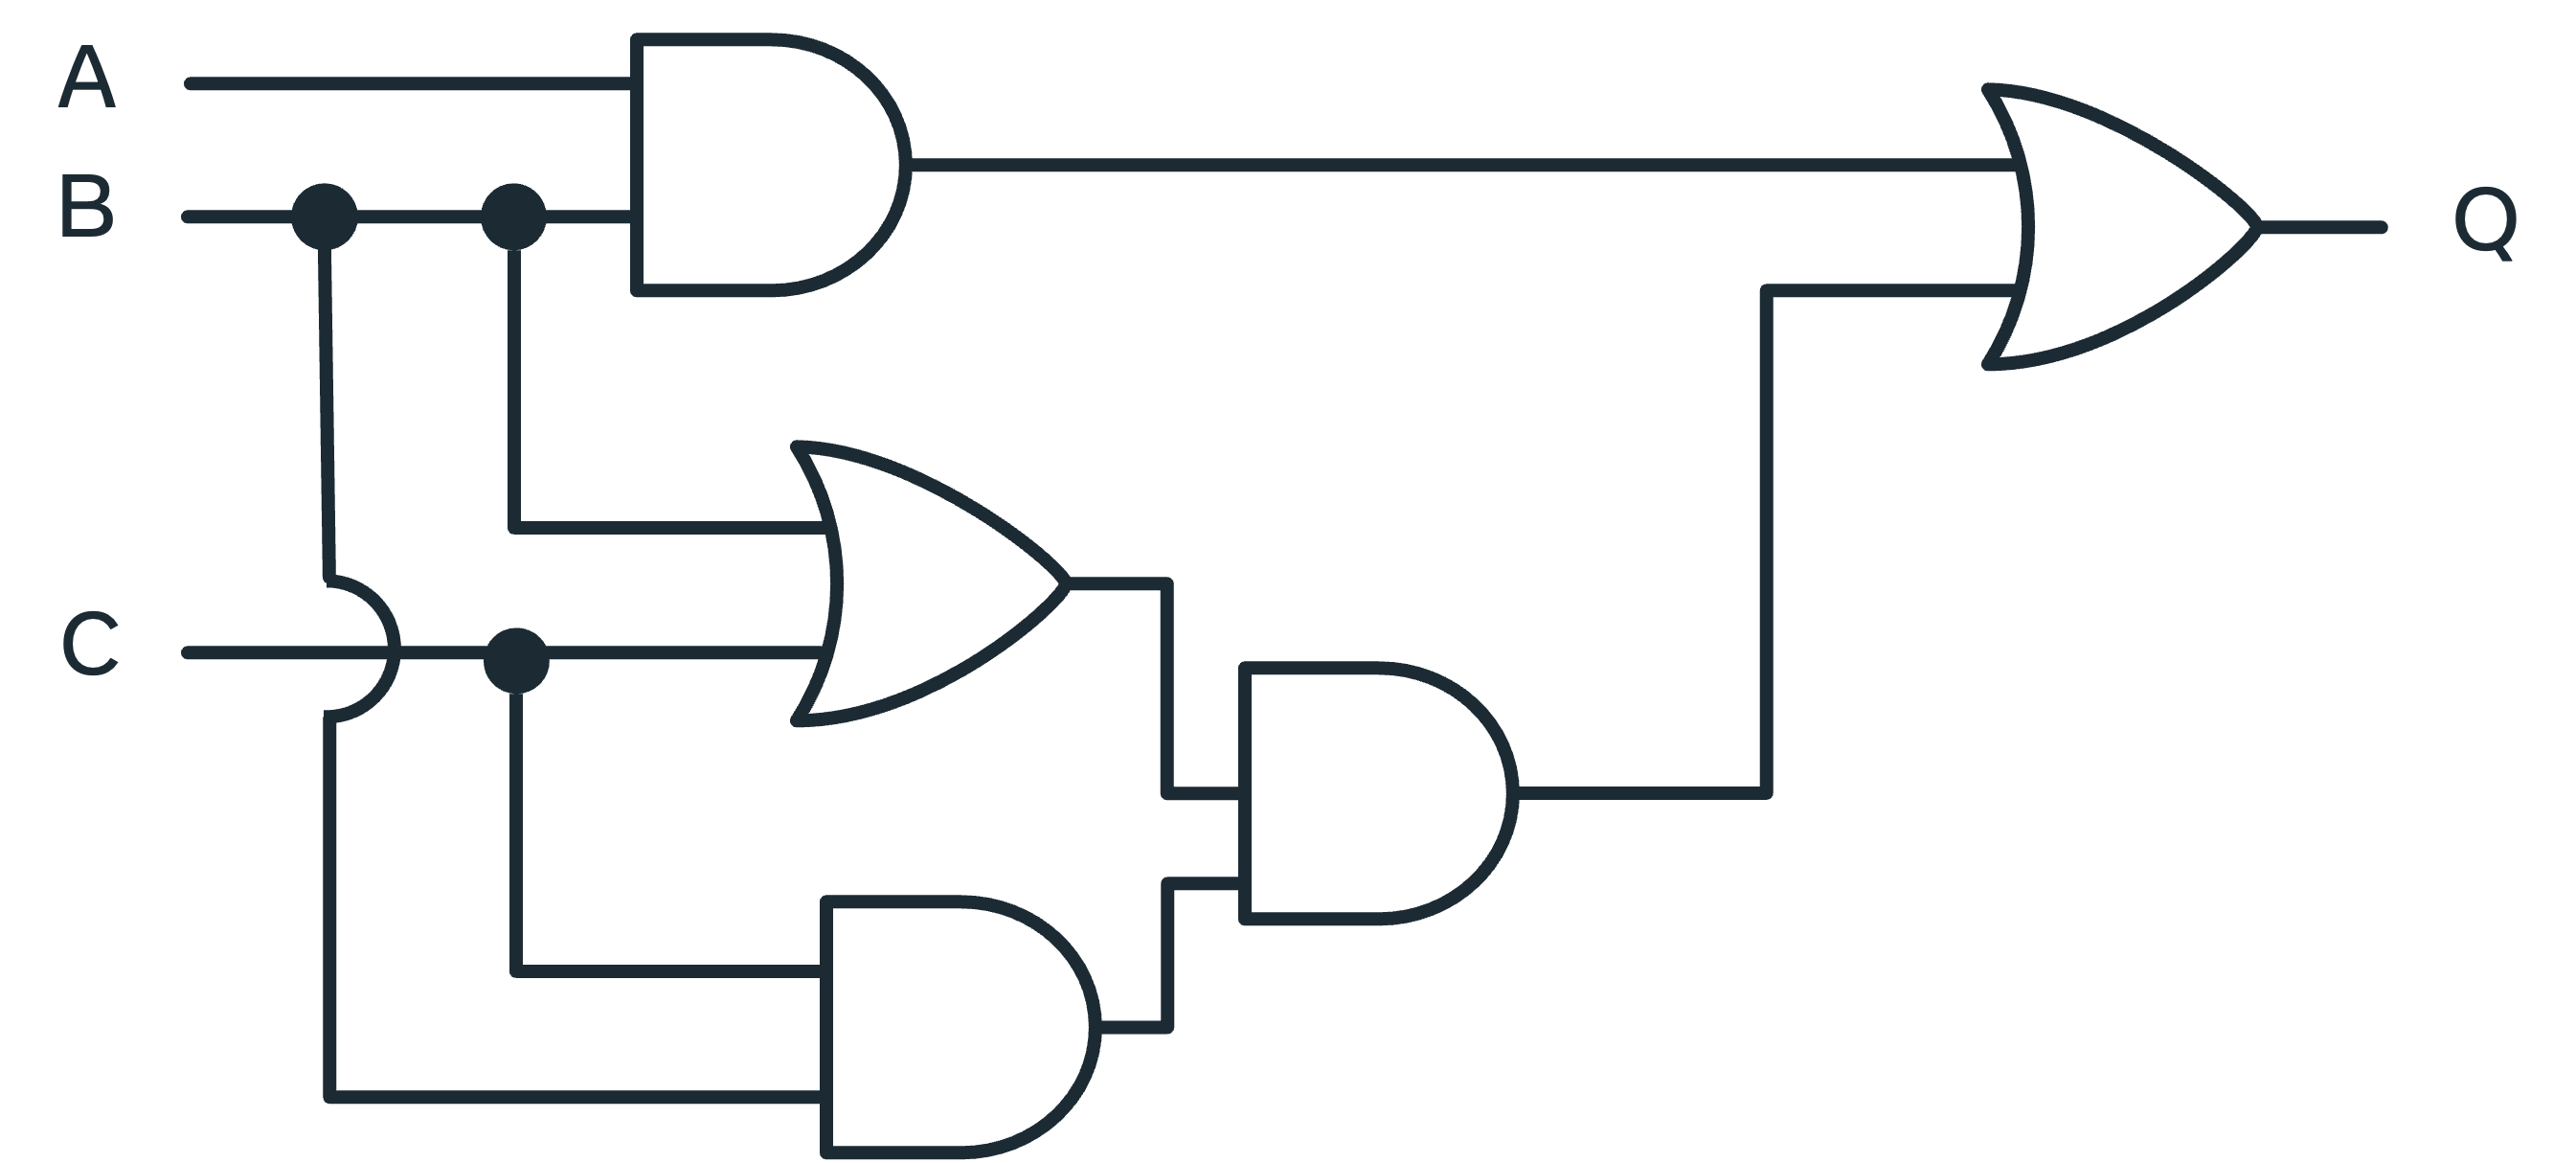
\includegraphics[width=0.8\textwidth]{./Picts/sirkuit.png}
    \caption{}
\end{figure}

\subsection{CPU dan Memori}
\begin{itemize}
    \item CPU (Central Processing Unit): Unit pemrosesan pusat yang mengolah informasi dan instruksi. CPU bekerja lebih cepat daripada kecepatan transfer informasi ke dalamnya.
    \item Memori: Terdiri dari blok-blok memori yang menyimpan informasi dan instruksi. Kapasitas memori mengacu pada jumlah bytes yang dapat disimpan oleh komputer.
\end{itemize}

\subsection{Jenis-jenis Memori}
\begin{itemize}
    \item Cache Memory: Memori termahal yang terletak dekat dengan CPU. Cache menyimpan informasi yang sering diakses untuk mempercepat proses. Jika informasi tidak ada di cache, CPU akan mencari di memori utama.
    \item Main Memory: Terdiri dari RAM (Random Access Memory) dan ROM (Read-Only Memory).

          \begin{itemize}
              \item RAM: Memori yang dapat diprogram dan menyimpan data serta instruksi yang sedang digunakan. Memori ini bersifat volatile, artinya data hilang saat daya mati.
              \item ROM: Memori yang hanya dapat dibaca dan tidak dapat diubah. Menyimpan instruksi penting untuk fungsi komputer.
          \end{itemize}
    \item Secondary Memory: Memori eksternal yang dapat ditambahkan untuk meningkatkan kapasitas penyimpanan. Contohnya termasuk cloud storage, hard drive eksternal, dan memory sticks. Akses ke memori sekunder lebih lambat karena memerlukan transfer informasi ke RAM terlebih dahulu.
\end{itemize}

\subsection{Pendekatan untuk Membuat Solusi di Komputer Sains}
Cara mendefinisikan solusi untuk pernyataan masalah dengan mengidentifikasi masalah, merumuskan model, dan menyempurnakan solusi.

\subsubsection{Mengidentifikasi masalah}
Langkah pertama dalam menyelesaikan suatu masalah adalah mengartikulasikannya. \textbf{Saya perlu mencapai tujuan A, dengan menggunakan alat T, dengan batasan C}. Untuk memperjelas konsep praktik terbaik dalam merancang solusi, mari kita pertimbangkan masalah dunia nyata. Misalnya, Anda harus merancang aplikasi yang akan menghibur anak dengan permainan tebak-tebakan. Secara sekilas, ini tampak seperti tugas yang sederhana: komputer + permainan = anak yang bahagia. Namun, sebelum memulai, ada baiknya menentukan beberapa detail.
\begin{itemize}
    \item Bagaimana anak akan berinteraksi dengan komputer?
    \item Pada tingkat apa pertanyaan-pertanyaan tersebut harus diajukan?
    \item Dari mana pertanyaan-pertanyaan tersebut dihasilkan?
    \item Bagaimana mereka akan disimpan?
    \item Bagaimana jawaban-jawaban tersebut akan diperiksa?
    \item Bagaimana program akan dimulai dan diakhiri?
\end{itemize}

Dalam skenario ini, masalahnya melibatkan baik perangkat keras maupun perangkat lunak. Pertama, apakah anak tersebut sudah cukup umur sehingga tidak memerlukan langkah-langkah keamanan? Dengan kata lain, penting untuk mempertimbangkan solusi ideal dengan memperhatikan bagaimana aplikasi akhir akan digunakan. Memberikan laptop mahal kepada balita mungkin bisa memberikan ketenangan sejenak, tetapi bisa saja menghabiskan gaji sebulan! Pola pikir yang sama harus diterapkan pada aplikasi yang direncanakan. Apakah pengguna akan mengakses aplikasi Anda dengan sinyal internet yang kuat? Apakah ada batasan lain, seperti output yang harus kompatibel dengan berbagai jenis ponsel? Apakah ada sistem operasi atau browser tertentu yang harus didukung? Semua pertanyaan ini perlu dipertimbangkan sebelum Anda mulai mengembangkan aplikasi.

\subsubsection{Merumuskan model}
Sekarang setelah ada gambaran tentang beberapa batasan proyek, solusi potensial dapat diusulkan. Bayangkan anak tersebut sudah cukup usia untuk menggunakan komputer, aplikasi hanya perlu dijalankan di laptop, semua penyimpanan dilakukan secara lokal (sehingga tidak ada masalah koneksi internet), dan input dapat dilakukan menggunakan keyboard di baris perintah. Bagus, sekarang proyek ini dapat dieksplorasi lebih lanjut.

Setelah menentukan ruang lingkup proyek, saatnya mempertimbangkan apa yang harus dilakukan oleh komputer. Algoritma dapat didefinisikan sebagai urutan instruksi yang tepat untuk memecahkan masalah. Berguna untuk terlebih dahulu menggeneralisasi masalah dan kemudian menggambarkan urutan instruksi yang diperlukan secara lebih rinci sebelum mengimplementasikan kode. Ini seperti mengambil pendekatan algoritmik untuk memecahkan masalah. Seorang programmer sering kali mendapatkan intuisi tentang bagaimana solusi seharusnya terlihat dengan terlebih dahulu menggambarkan masalah menggunakan pseudocode. Ini dapat berupa deskripsi teks yang merinci persyaratan.

\begin{figure}[H]
    \centering
    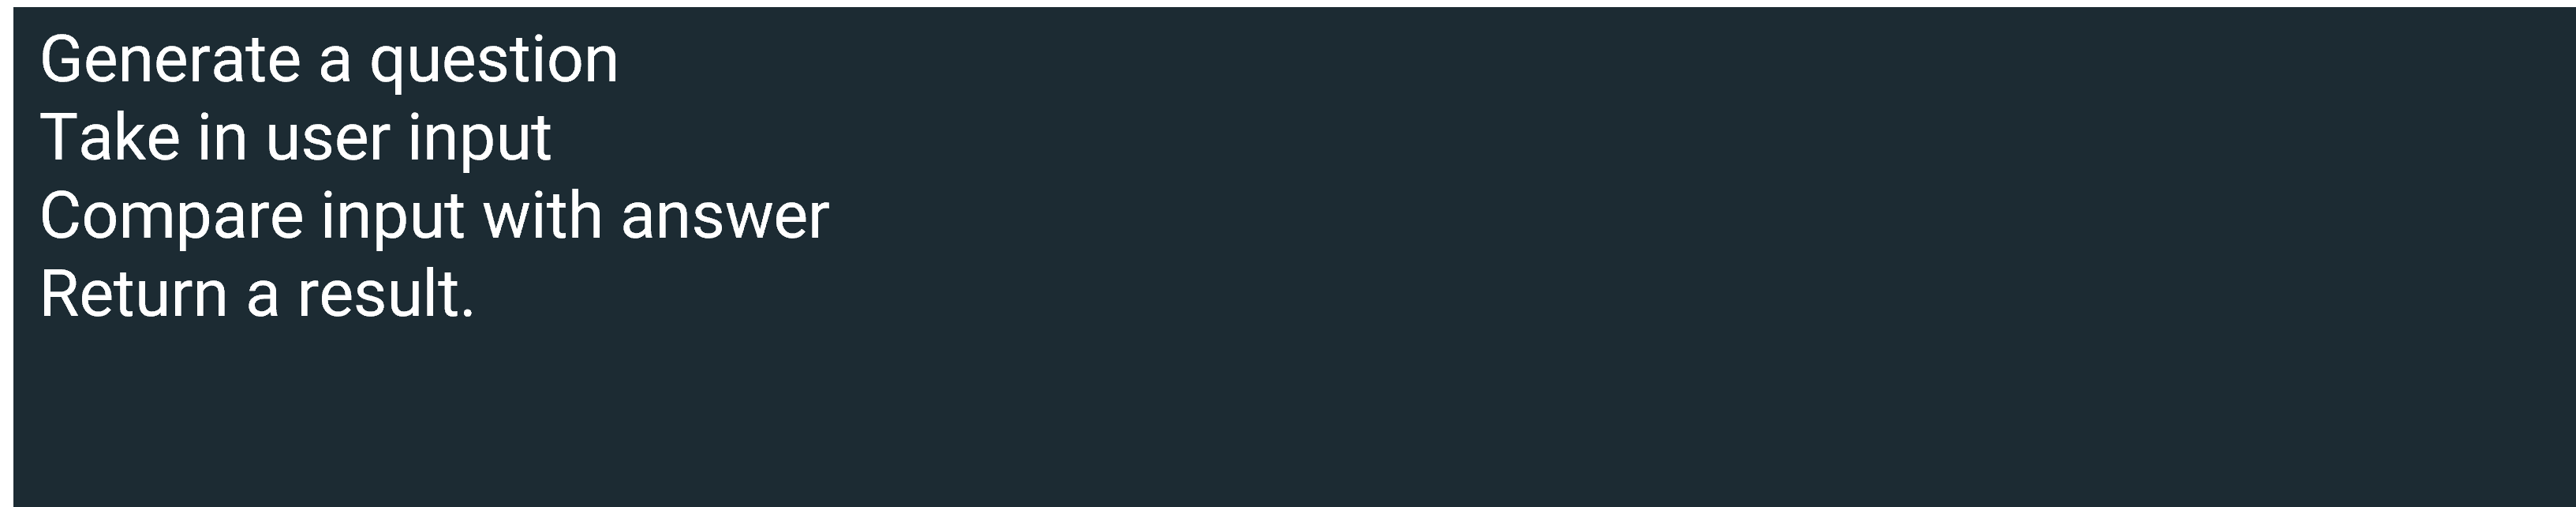
\includegraphics[width=0.8\textwidth]{./Picts/fthemodel.png}
    \caption{}
\end{figure}

Menyusun langkah-langkah dalam daftar adalah langkah awal yang baik. Sekarang, pertimbangkan cara menghasilkan pertanyaan yang sesuai dengan usia. Menghasilkan pertanyaan secara dinamis dari ensiklopedia online atau sumber online lainnya mungkin memakan waktu. Sebagai alternatif, Anda dapat mengidentifikasi sumber pertanyaan dan jawaban yang sudah dikompilasi.

Kedua, bagaimana masukan pengguna diambil? Telah ditetapkan bahwa keyboard adalah opsi yang layak, tetapi seberapa mahir anak dalam mengetik? Membandingkan solusi dengan teks memiliki tantangannya sendiri. Apakah harus cocok secara langsung, apakah ejaan, tanda baca, dan huruf besar akan dipertimbangkan? Potensial, pertanyaan dapat berupa pilihan ganda. Meningkatkan kesadaran akan semua pertimbangan ini adalah tujuan dari merumuskan pernyataan masalah secara jelas daripada langsung melompat ke solusi.

\subsubsection{Menyempurnakan solusi}
Setelah mempertimbangkan dengan matang, Anda menyadari bahwa pendekatan pengetahuan dasar akan menimbulkan terlalu banyak hambatan, sehingga proyek ini didefinisikan ulang sebagai permainan menebak angka. Permainan ini cocok untuk semua usia dan tidak memerlukan sumber daya eksternal. Selain itu, permainan ini seharusnya dapat diimplementasikan dengan sebagian besar bahasa pemrograman.
\begin{figure}[H]
    \centering
    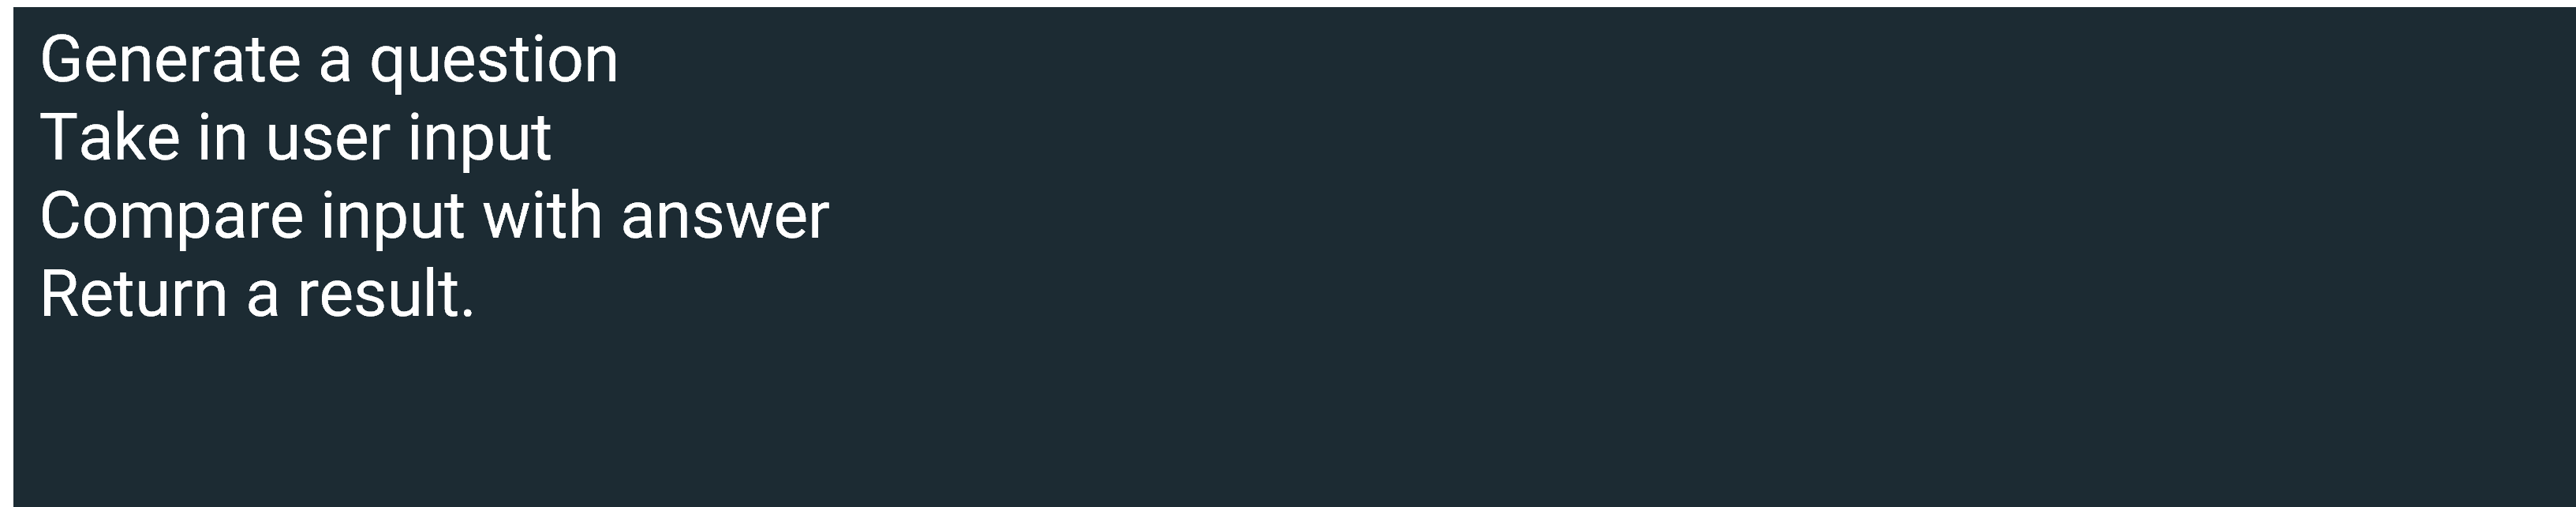
\includegraphics[width=0.8\textwidth]{./Picts/fthemodel.png}
    \caption{}
\end{figure}

Setelah menjelaskan persyaratan umum, kita dapat menguraikan detail-detailnya. Di bawah ini adalah diagram alir pseudocode, yang dapat memberikan wawasan lebih lanjut tentang cara terbaik untuk merumuskan solusi.

\begin{figure}[H]
    \centering
    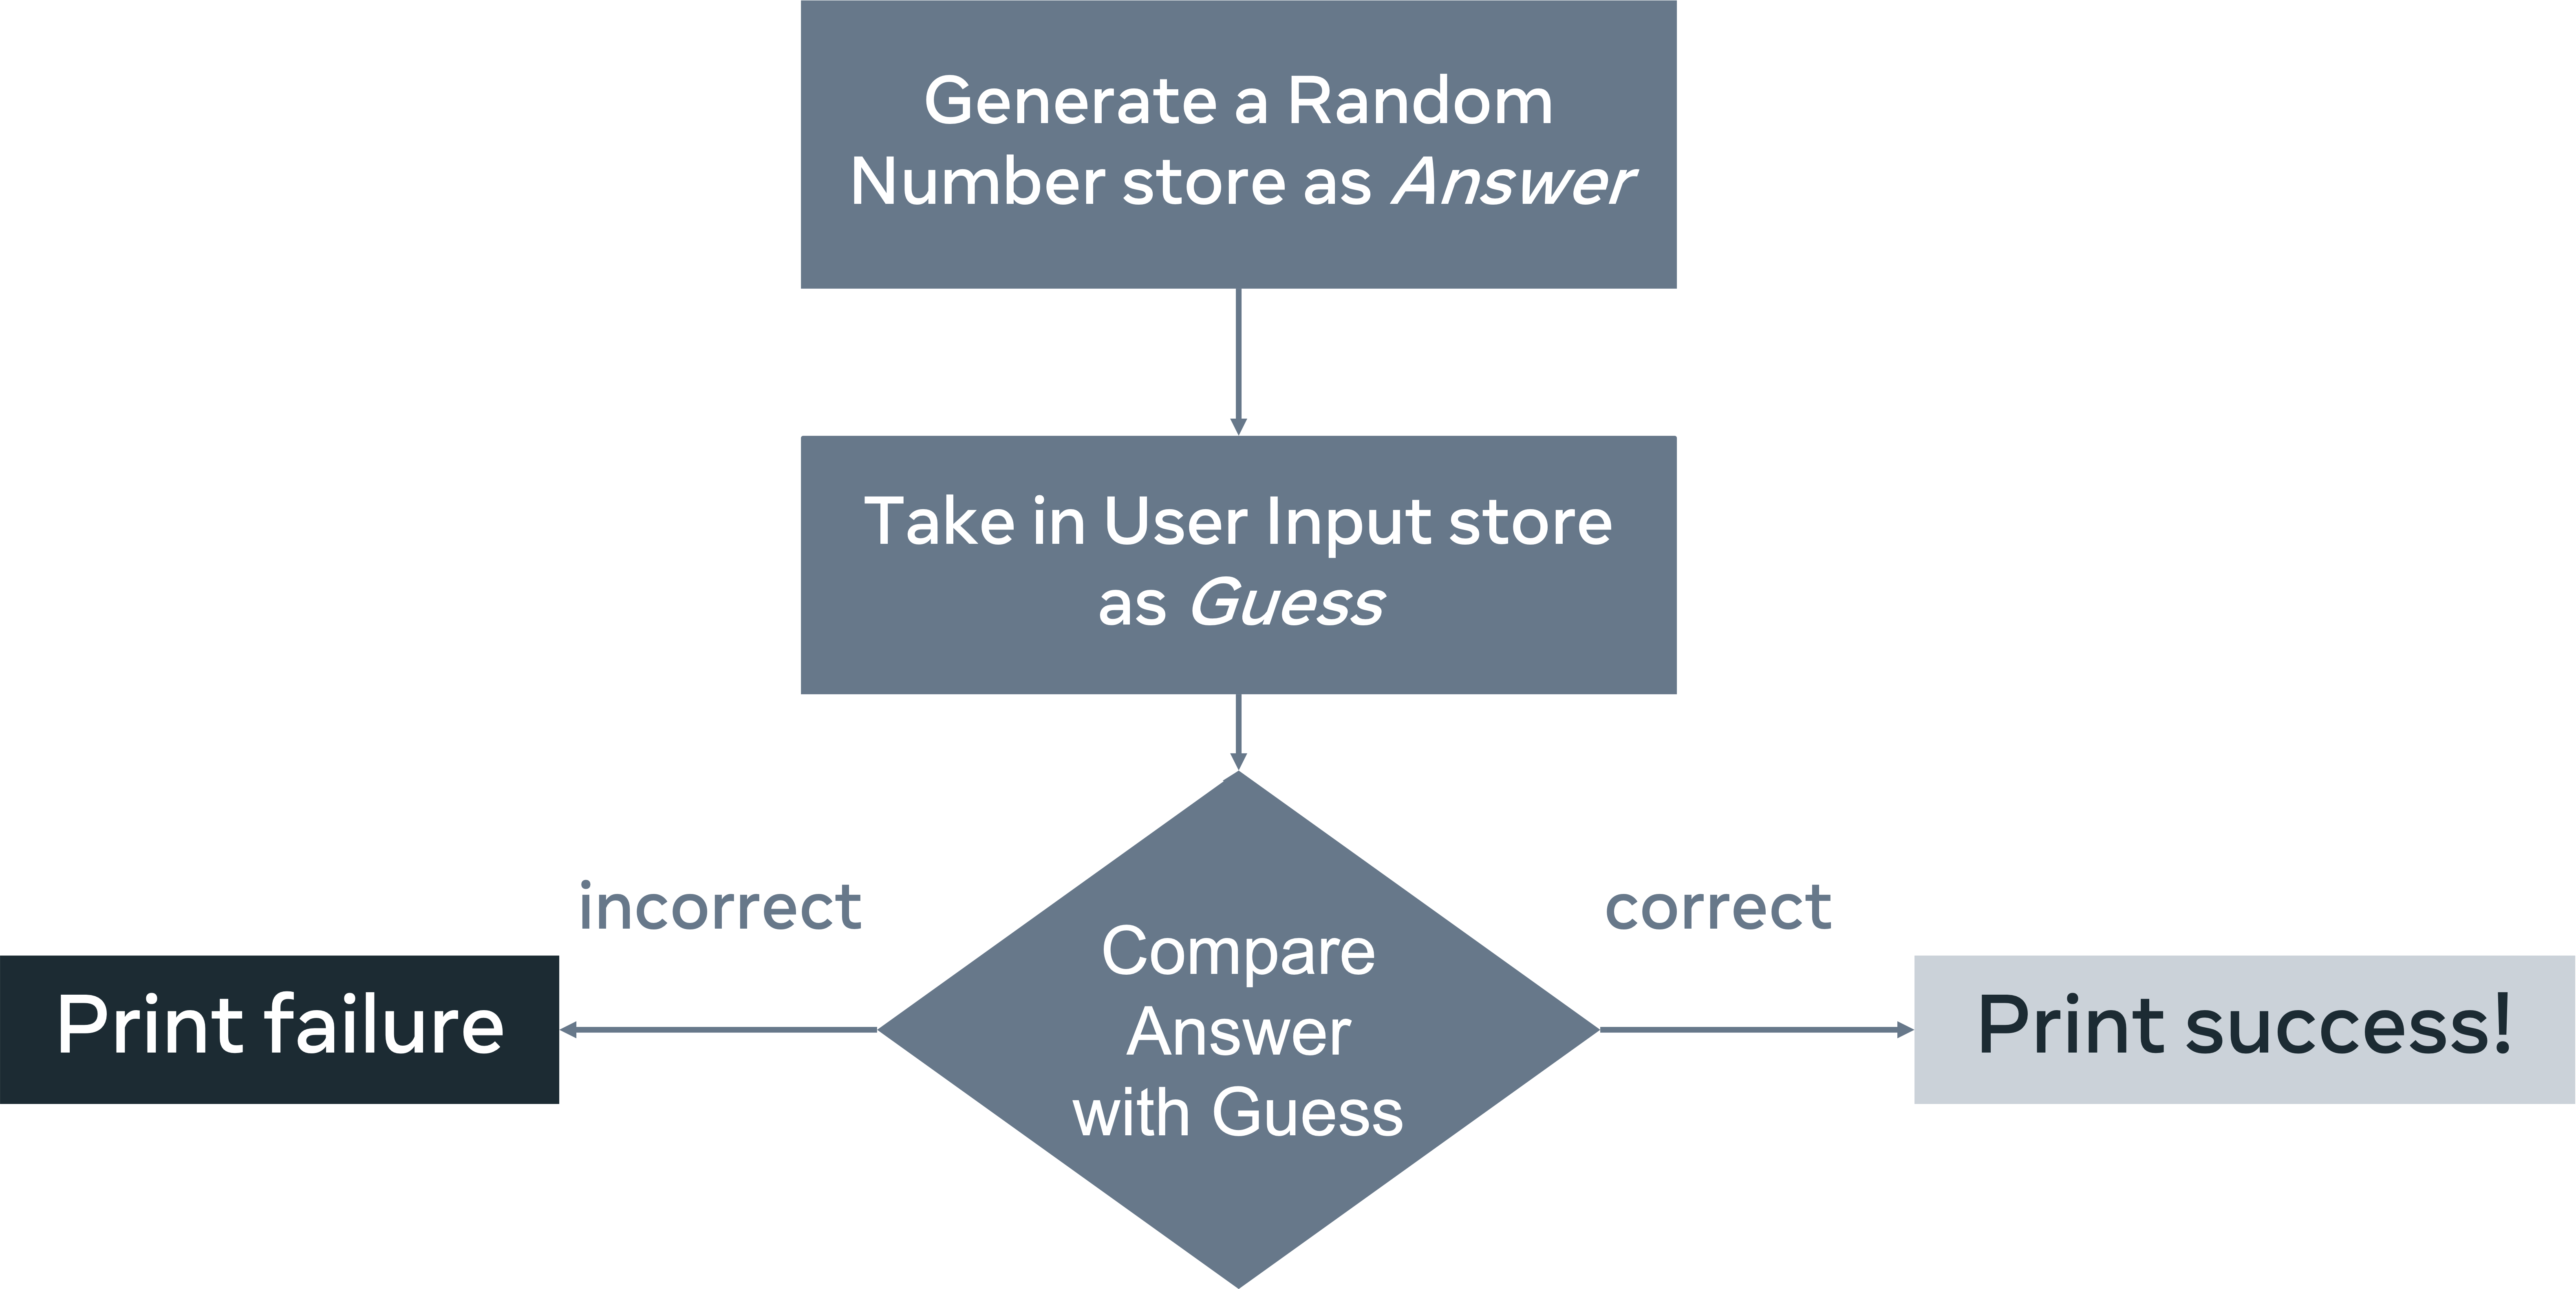
\includegraphics[width=0.8\textwidth]{./Picts/flowchart1.png}
    \caption{}
\end{figure}

Menganalisis diagram alir mengidentifikasi pertimbangan tambahan. Apakah program akan dijalankan hanya sekali? Apa yang dapat ditambahkan untuk meningkatkan pengalaman pengguna? Menampilkan pesan kegagalan mungkin bukan output yang ideal. Sebagai gantinya, opsi yang mungkin adalah memberikan kesempatan lain untuk menebak. Pertimbangan tambahan lainnya adalah menyediakan petunjuk yang dapat digunakan untuk mengarahkan pengguna ke jawaban yang benar. Dan, Anda harus memutuskan apa yang terjadi jika pengguna memasukkan nilai non-angka ke dalam program.

\begin{figure}[H]
    \centering
    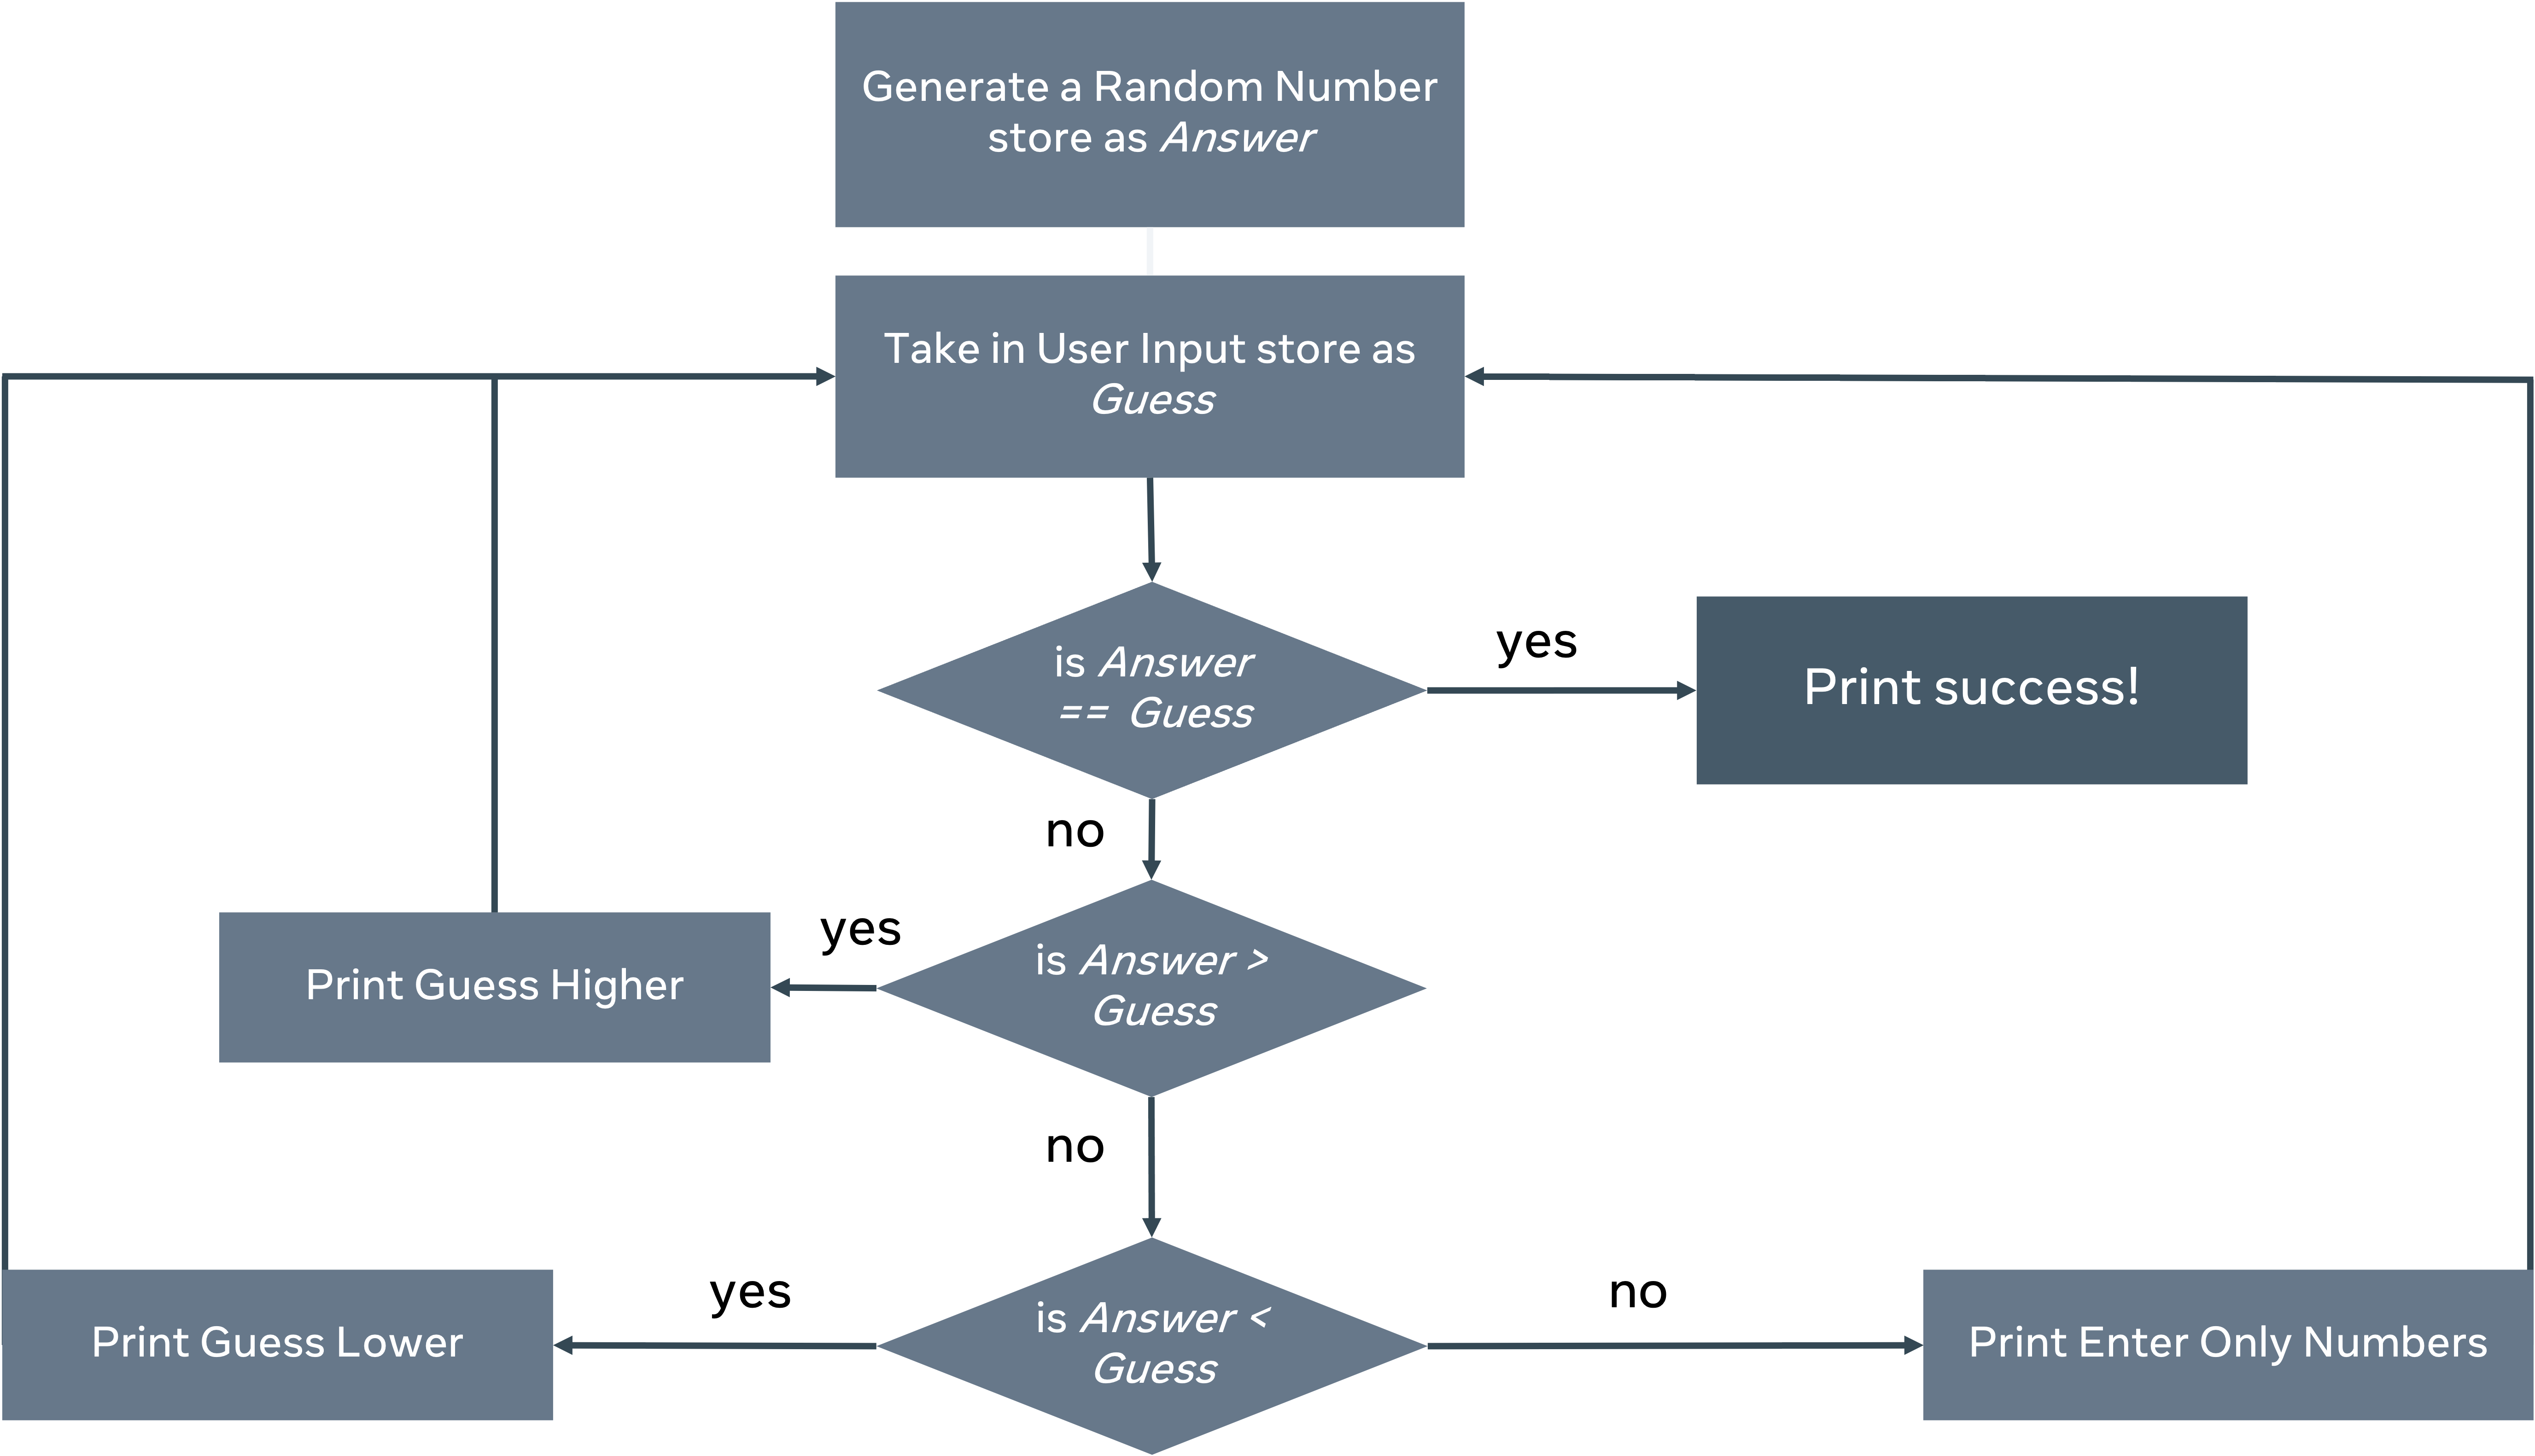
\includegraphics[width=0.8\textwidth]{./Picts/flowchart2.png}
    \caption{}
\end{figure}

Sekarang setelah berbagai kondisi telah dijelaskan, kita dapat memilih bahasa pemrograman dan mengimplementasikan solusi. Dengan mengambil pendekatan sistematis dalam pemecahan masalah, Anda telah mengidentifikasi beberapa masalah potensial sebelum proyek dimulai dan dapat melakukan penyesuaian arah. Setelah mengevaluasi solusi, cakupan proyek mungkin perlu diubah. Alih-alih membuat permainan untuk diimplementasikan oleh anak, program tersebut mungkin akan menciptakan lingkungan sehingga anak dapat membuat permainan sendiri, menggunakan deskripsi yang jelas sebagai panduan.

\subsection{Evaluasi Time Complexity}
\begin{itemize}
    \item Kompleksitas Waktu (Time Complexity): Ukuran seberapa lama algoritma akan berjalan berdasarkan ukuran input. Ini penting untuk memastikan aplikasi memberikan respons dalam waktu yang dapat diterima.
    \item Notasi Big-O (Big-O Notation): Metode untuk menggambarkan kompleksitas waktu algoritma. Contoh notasi yang umum termasuk O(1), O(log n), O(n), dan O(n²).
\end{itemize}

\subsection{Contoh Kompleksitas Waktu}
\begin{itemize}
    \item O(1): Algoritma yang memerlukan waktu konstan untuk menyelesaikan tugas, terlepas dari ukuran input. Contoh: mencetak item pertama dalam array.
    \item O(n): Algoritma yang memerlukan waktu linear, di mana waktu yang dibutuhkan sebanding dengan ukuran input. Contoh: mencari nilai dalam array dengan memeriksa setiap item.
    \item O(log n): Algoritma yang lebih efisien daripada O(n), di mana waktu yang dibutuhkan meningkat secara marginal dengan bertambahnya input. Contoh: pencarian biner (binary search).
    \item \(O(n^2)\): Algoritma dengan kompleksitas kuadratik, di mana waktu yang dibutuhkan berlipat ganda untuk setiap elemen dalam array. Contoh: algoritma yang melibatkan dua loop yang masing-masing berjalan sebanyak n kali.
\end{itemize}

\subsection{Kasus Terbaik, Terburuk, dan Tengah}
Walau O(n) melekat pada loop, tapi loop tidak selalu menghasilkan kompleksitas waktu tersebut, dan dapat memiliki 3 opsi:
\begin{itemize}
    \item Kasus Terbaik (Best Case): Situasi di mana algoritma menyelesaikan tugas dengan waktu paling cepat. Contohnya ketika apa yang dicari sudah ditemukan di awal array, maka notasinya adalah O(1)
    \item Kasus Terburuk (Worst Case): Situasi di mana algoritma memerlukan waktu paling lama untuk menyelesaikan tugas. Ini jika yang dicari tidak ditemukan, maka loop akan berjalan sampai akhir, dan inilah O(n)
    \item Kasus Rata-rata (Average Case): Waktu yang diharapkan untuk menyelesaikan tugas dalam situasi umum. Ini jika loop sudah bisa diberhentikan di tengah array, O(n/2).
\end{itemize}

\subsection{Pertanyaan untuk Evaluasi}
Sebelum memulai, tanyakan pada diri sendiri: "Berapa banyak komputasi yang digunakan solusi saya? Apakah ada cara yang lebih baik?"

\subsection{Bekerja dengan Kompleksitas Waktu}
\subsubsection{Pendahuluan}
Evaluasi kinerja aplikasi memastikan bahwa kode yang ditulis baik dan sesuai dengan tujuannya. Pertanyaannya adalah bagaimana kita mengevaluasi efisiensi? Saat mengukur listrik, kita menggunakan kilowatt-jam, yang berarti berapa banyak kilowatt yang akan digunakan oleh suatu perangkat jika dijalankan selama satu jam. Perangkat tersebut tidak selalu dijalankan selama satu jam, dan mungkin memiliki persyaratan yang berbeda tergantung pada pengaturan yang digunakan, ini lebih merupakan pedoman umum untuk mengevaluasi biaya.

Saat mengevaluasi solusi pemrograman, notasi Big-O digunakan. Jadi, notasi Big-O adalah kilowatt-jam dalam evaluasi kode. Notasi ini dapat diterapkan untuk mengukur berapa lama waktu yang dibutuhkan oleh sepotong kode atau berapa banyak ruang yang akan digunakan di memori. Tidak semua prosesor berjalan dengan kecepatan yang sama, jadi daripada mengukur waktu aplikasi, kita menghitung jumlah instruksi yang diinisialisasi oleh aplikasi.

\subsubsection{Mana Pengukuran yang Benar Merefleksikan Kemungkinan Eksekusi yang Paling Cepat dari Sebuah Kode?}
Mari kita telusuri pengukuran mana yang mencerminkan eksekusi kode tercepat yang mungkin.

\paragraph{O(1)}

Anda menggunakan algoritma waktu konstan yang membutuhkan waktu O(1) (O-dari-satu) untuk dihitung. Hal ini menentukan bahwa hanya diperlukan satu kali perhitungan untuk menyelesaikan suatu tugas. Contohnya adalah mencetak suatu elemen dari sebuah array dengan indeks.
\begin{lstlisting}[language=Python, caption={}, captionpos=b]
# An array with 5 numbers 
array = [0,1,2,3,4]

# retrieve the number found at index location 3 
print(array[3]) 
\end{lstlisting}

Dalam hal ini, terlepas dari berapa banyak nilai yang ada dalam array, pendekatan ini memiliki kompleksitas Big-O sebesar satu. Artinya, menjalankan kode ini dianggap memiliki kompleksitas O(1).

\paragraph{O(n)}

Selanjutnya, mari kita lihat contoh dari O(n). Menggunakan array yang sama, ditulis pernyataan if yang mencari angka 5. Untuk memastikan bahwa 5 tidak ada di sana, pernyataan tersebut harus memeriksa setiap elemen dalam array.
\begin{lstlisting}[language=Python, caption={}, captionpos=b]
# An array with 5 numbers 
array = [0,1,2,3,4] 

if 5 in array:
    print("five is alive")
\end{lstlisting}

Dalam contoh di atas, tidak ada angka 5, jadi tidak ada hasil cetak. Untuk memastikan hal ini, dilakukan lima pemeriksaan pada array ini. Karena input n = 5, kode ini dikatakan memiliki kompleksitas Big-O sebesar O(n). Untuk memahami hal ini dengan lebih baik, mari kita perpanjang array menjadi 10 dan menghilangkan angka 5.
\begin{lstlisting}[language=Python, caption={}, captionpos=b]
# an array with 10 numbers 
array = [0,1,2,3,4,6,7,8,9,10]

if 5 in array:
    print("five is still alive")
\end{lstlisting}

Dengan memperluas array menjadi 10 bilangan bulat, jumlah perhitungan kini menjadi 10. Hal ini masih disebut O(n) karena ukuran inputnya adalah 10, yang merupakan jumlah pemeriksaan yang harus dilakukan sebelum program berakhir.

\paragraph{O(log n)}

Pencarian ini kurang intensif daripada O(n) tetapi lebih banyak kerja daripada O(1). O(log n) adalah pencarian logaritmik dan akan meningkat seiring penambahan input baru, tetapi penambahan input ini hanya memberikan peningkatan marginal. Contoh yang sangat baik dari hal ini adalah pencarian biner. Pencarian biner dibahas lebih detail di bagian selanjutnya dalam kursus ini.

Sekarang, bayangkan bermain permainan tebak-tebakan dengan petunjuk berikut: terlalu tinggi, terlalu rendah, atau benar. Anda diberikan rentang 100 hingga 1. Anda mungkin memutuskan untuk mendekati masalah ini secara sistematis. Pertama, Anda menebak 50 – terlalu tinggi. Jadi, Anda menebak 25 – yang juga terlalu tinggi. Anda mungkin memilih untuk melanjutkan ke 12 atau 13. Yang terjadi di sini adalah Anda membagi dua ruang pencarian dengan setiap tebakan.

Jadi, meskipun input untuk fungsi ini adalah 100 menggunakan pendekatan pencarian biner, Anda seharusnya dapat menemukan jawabannya dalam kurang dari 5 atau 6 tebakan. Solusi ini memiliki kompleksitas waktu O(log n). Bahkan jika n (rentang angka yang dimasukkan) sepuluh kali lebih besar, jumlah tebakan yang diperlukan tidak akan sepuluh kali lipat.

Berikut ini adalah rincian langkah-langkah tersebut pada array.
\begin{lstlisting}[language=Python, caption={}, captionpos=b]
array = [0,1,2,3,4,6,7,8,9,10]

print("##Step One")
print("Array")
print(array)
midpoint = int(len(array)/2)
print("the midpoint at step one is: " , array[midpoint])

print()

print("##Step Two")
array = array[:midpoint] # 6 is the midpoint of the array 
print("Array")
print(array)
# running this shows the numbers left to check 
# is 5 < 3 
# no 
# so discard the left hand side 

# so the array is halved again 
midpoint=int(len(array)/2)
print("the midpoint is: ",  array[midpoint])

print()
print("##Step Three") 
array = array[midpoint:] # so the array is halved at the midpoint
print(array)
# check for the midpoint 
midpoint=int(len(array)/2)
print("the midpoint is: " , array[midpoint])
# is 4 < 5 
# yes look to the right

print()
print("##Step Four") 
print(array[midpoint:]) 
# check for the midpoint 
array = array[midpoint:] # so the array is halved at the midpoint
midpoint=int(len(array)/2)



print()
print("##Step Five") 
array = array[midpoint:] 
print(array)
print("only one value to check and it is not 5")
\end{lstlisting}

Outputnya:
\begin{lstlisting}[language=Python, caption={}, captionpos=b]
##Step One
Array
[0, 1, 2, 3, 4, 6, 7, 8, 9, 10]
the midpoint at step one is:  6

##Step Two
Array
[0, 1, 2, 3, 4]
the midpoint is:  2

##Step Three
[2, 3, 4]
the midpoint is:  3

##Step Four
[3, 4]

##Step Five
[4]
only one value to check and it is not 5
\end{lstlisting}

Anda akan menyadari bahwa untuk menentukan apakah angka 5 ada, diperlukan 5 langkah. Itu adalah skor Big-O sebesar O(5). Anda dapat melihat bahwa ini lebih besar dari O(1) tetapi lebih kecil dari O(n). Sekarang, apa yang terjadi jika array diperluas menjadi 100? Saat mencari angka dalam array berukuran 10, diperlukan 5 tebakan. Memeriksa array berukuran 100 tidak akan membutuhkan 50 tebakan; paling banyak hanya 10. Demikian pula, jika daftar diperluas menjadi 1000, tebakan hanya akan mencapai 15-20.

Dari ini, kita dapat melihat bahwa kompleksitasnya bukan O(1) karena jawaban tidak langsung diperoleh. Kompleksitasnya juga bukan big-O(n) karena jumlah tebakan tidak meningkat seiring dengan ukuran n dari array. Oleh karena itu, di sini dikatakan bahwa kompleksitasnya adalah O(log(n)).

Untuk mendapatkan pemahaman yang lebih mendalam tentang bagaimana nilai logaritma hanya mengalami kenaikan secara bertahap, lihat tabel logaritma hingga 100.000.000. Perspektif ini menunjukkan bahwa O(log n) hanya menimbulkan biaya pemrosesan yang minimal. Melakukan pencarian biner pada array dengan n nilai apa pun, dalam skenario terburuk, akan selalu menghasilkan jumlah perhitungan yang tercantum dalam kolom nilai logaritma.

\begin{figure}[H]
    \centering
    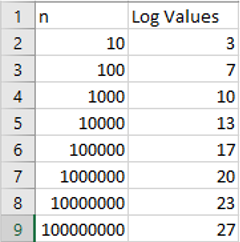
\includegraphics[width=0.8\textwidth]{./Picts/logntabel.png}
    \caption{}
\end{figure}

\paragraph{\(O(n^2)\)}

memiliki beban komputasi yang tinggi. Ini adalah kompleksitas kuadratik, artinya jumlah operasi yang diperlukan tumbuh secara proporsional dengan kuadrat ukuran input. Sebuah array berukuran n akan memiliki jumlah operasi total sekitar \(n^2\). Cara yang baik untuk memvisualisasikan ini adalah dengan mempertimbangkan bahwa Anda memiliki berbagai array. Mengikuti contoh sebelumnya, mari kita jelajahi kode berikut:
\begin{lstlisting}[language=Python, caption={}, captionpos=b]
new_array=[] # an array to hold all of the results 
# array with five numbers 
array = [0,1,2,3,4]
for i in range(len(array)): # the array has five values, so this is n=5 
    for j in range(len(array)): # still the same array so n = 5 
        new_array.append(i*j) # every computation made is stored here 

print(len(new_array)) #how big is this new array ? 
\end{lstlisting}

Lingkaran pertama akan sama dengan jumlah elemen input, n. Lingkaran kedua juga akan memeriksa jumlah elemen input, n. Oleh karena itu, kompleksitas keseluruhan dari pendekatan ini dapat dikatakan sebagai \(n*n\), yang merupakan \(n^2\) (n kuadrat). Untuk mengetahui berapa banyak perhitungan yang dilakukan, Anda harus mencetak jumlah kali n digunakan dalam lingkaran seperti di bawah ini.

\begin{lstlisting}[language=Python, caption={}, captionpos=b]
n = 5 #size of array 
print(n*n) # how big is this new array ? 
\end{lstlisting}

\(O(n^2)\) memiliki beban komputasi yang tinggi. Ini adalah kompleksitas kuadratik, artinya jumlah operasi yang diperlukan tumbuh secara proporsional dengan kuadrat ukuran input. Sebuah array berukuran n akan memiliki jumlah operasi total sekitar n². Cara yang baik untuk memvisualisasikan ini adalah dengan mempertimbangkan bahwa Anda memiliki berbagai array. Mengikuti contoh sebelumnya, mari kita jelajahi kode berikut:

\subsubsection{Representasi Visual dari Sebuah Masalah}
Di bawah ini adalah representasi grafis yang menunjukkan hubungan antara n dengan jumlah perhitungan yang diperlukan.
\begin{figure}[H]
    \centering
    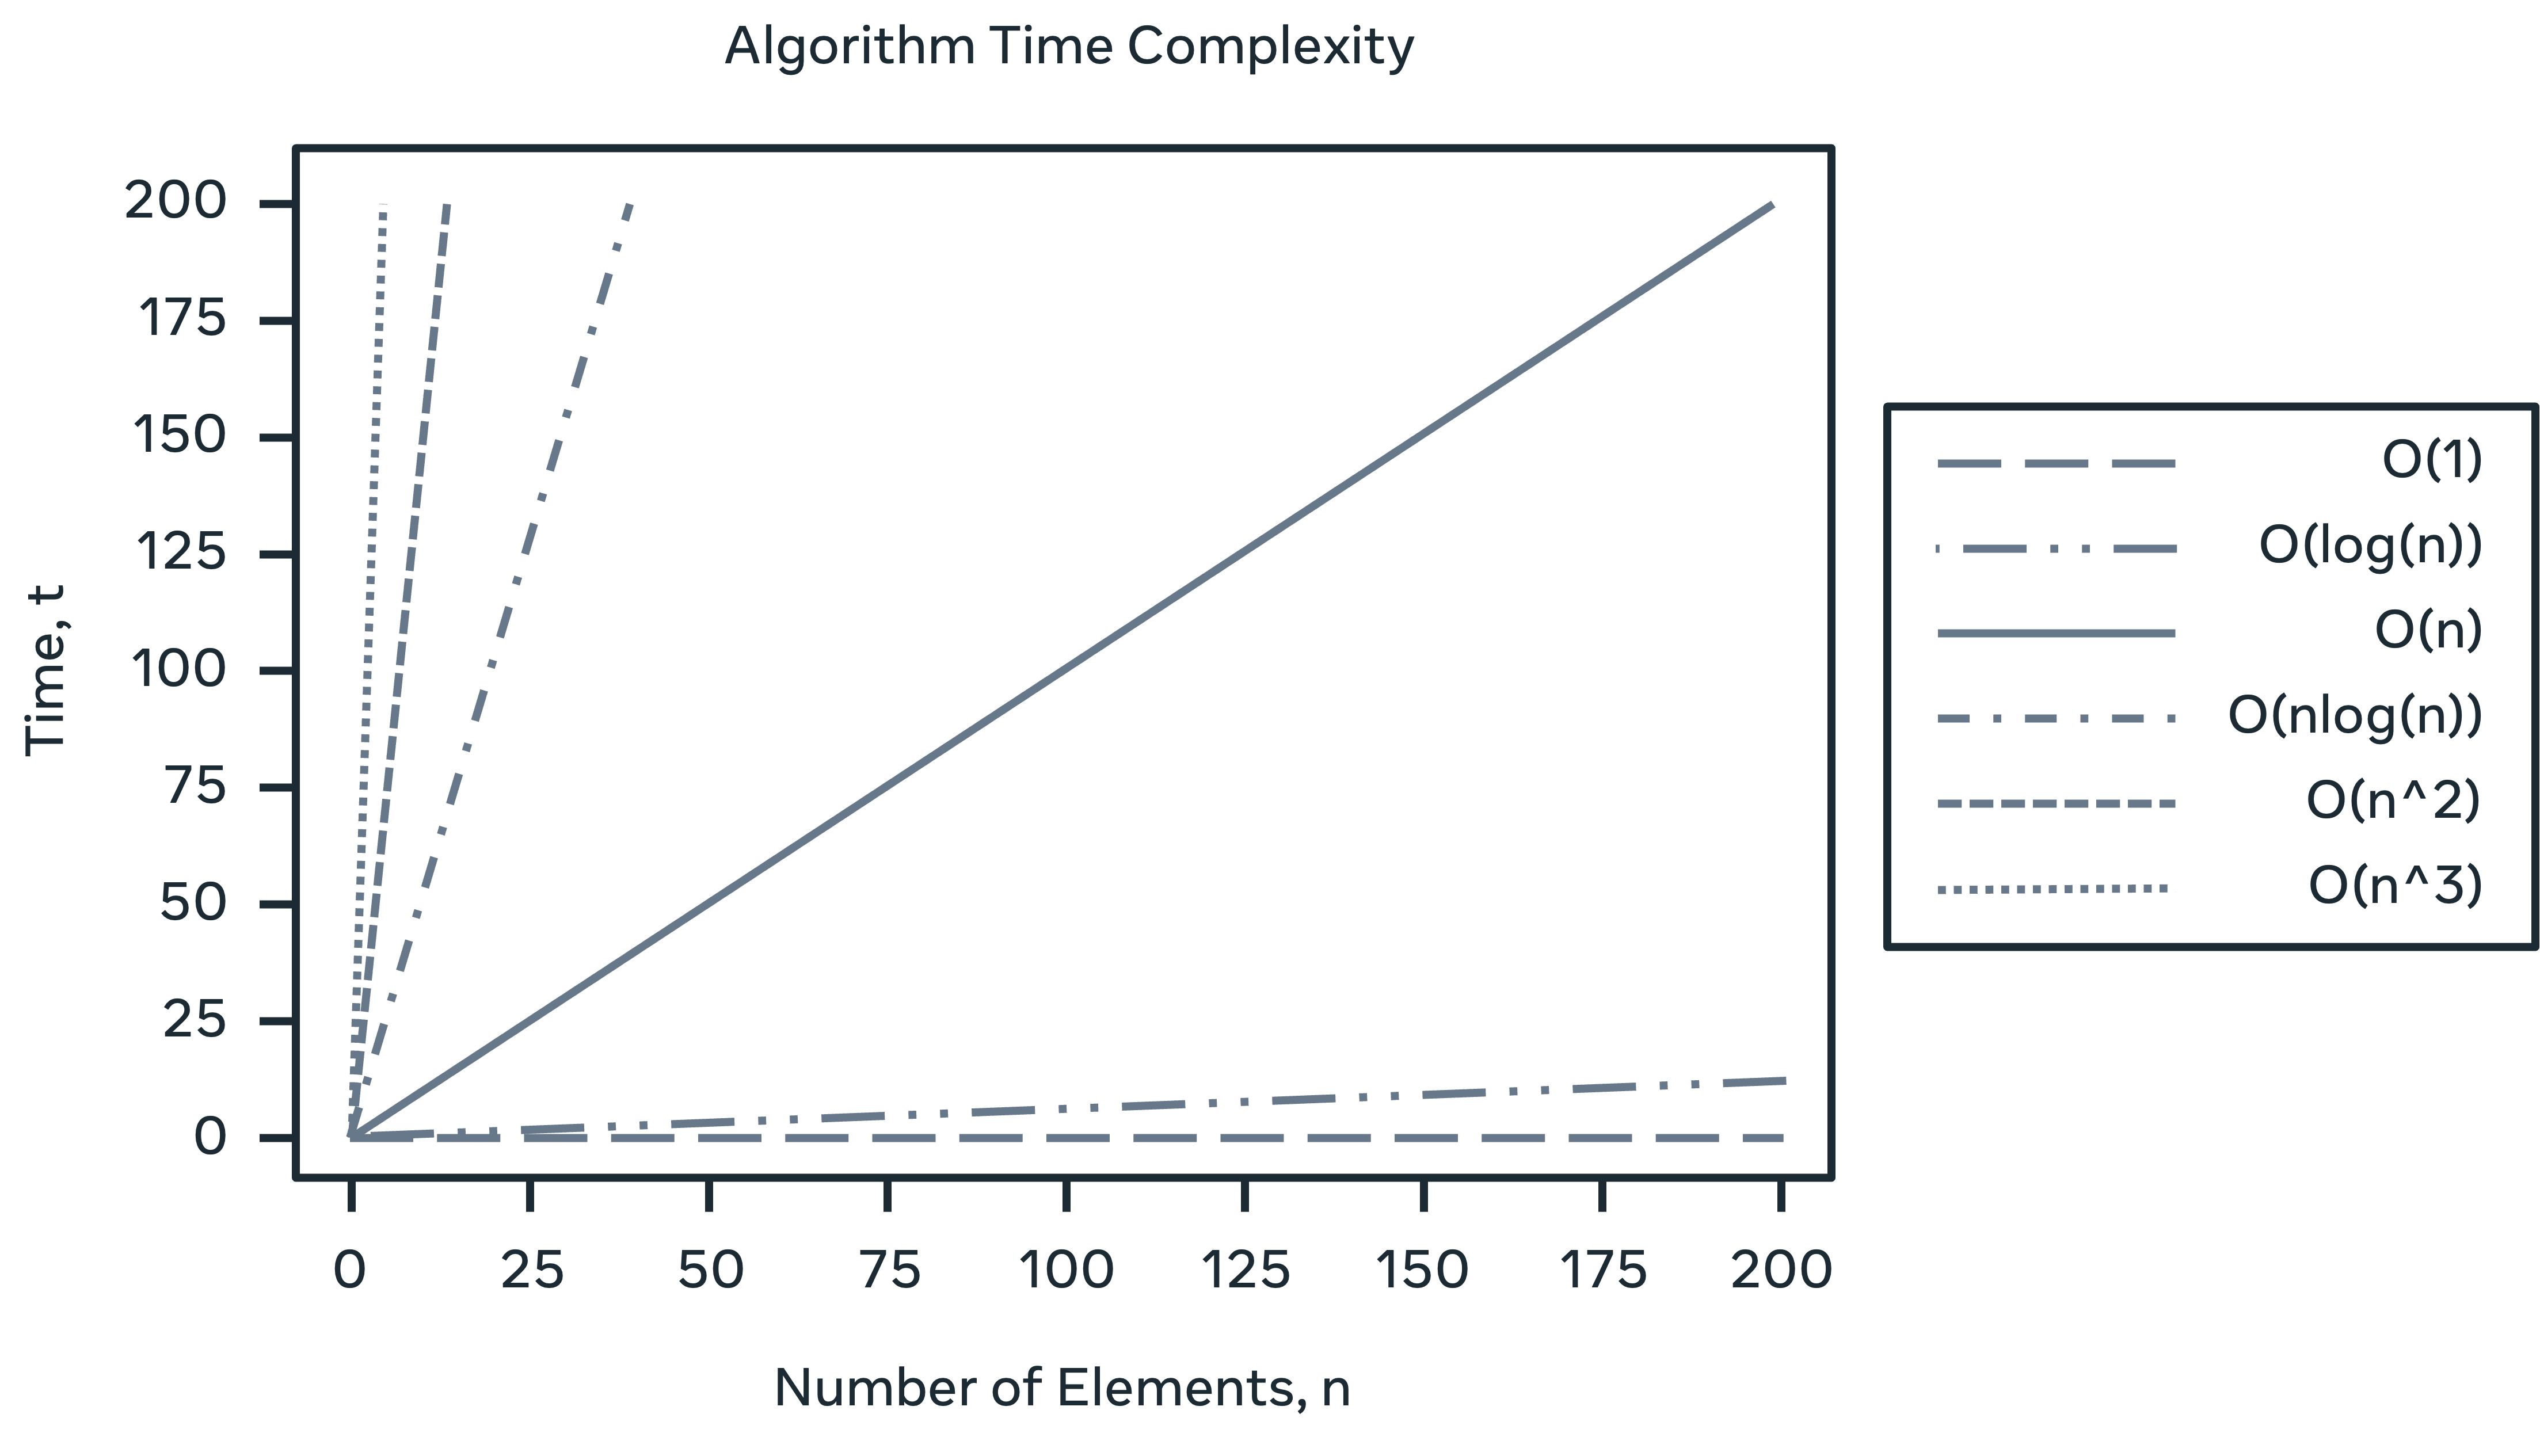
\includegraphics[width=0.8\textwidth]{./Picts/vreptimecomp.png}
    \caption{}
\end{figure}

Seperti yang dapat Anda lihat, waktu terbaik yang harus dituju adalah O(1); O(log n) masih sangat baik. O(n) masih bisa diterima, sedangkan\(O(n^2)\) tidak terlalu baik.

\subsubsection{Kasus buruk, Kasus baik, dan Kasus rata-rata}
Tentu saja, tidak selalu mungkin untuk mengetahui berapa lama suatu pendekatan akan memakan waktu. Ketika melihat contoh loop awal, terdapat pencarian yang dilakukan untuk elemen yang tidak ada. Anda dapat mengatakan bahwa mencari dalam loop memakan waktu O(n), tetapi hal ini tidak selalu berlaku.

Pertimbangkan bahwa elemen yang dicari adalah elemen pertama dalam array. Maka waktu kembalinya akan cukup baik dalam O(1) waktu! Dalam contoh yang diberikan, setiap elemen harus dicari sebelum menentukan bahwa elemen tersebut tidak ada: O(n) waktu. Kasus tengah adalah ketika elemen tersebut ditemukan di tengah loop: O(n/2). Saat mengevaluasi suatu pendekatan, tiga definisi digunakan: kasus terbaik, kasus terburuk, dan kasus rata-rata.

\subsection{Konsep Dasar}
\begin{itemize}
    \item Kompleksitas Ruang: Mengukur seberapa banyak memori yang dibutuhkan oleh algoritma untuk menyelesaikan masalah, sering kali menjadi trade-off dengan waktu eksekusi.
    \item Big-O Notation: Notasi yang digunakan untuk menggambarkan kompleksitas ruang, seperti O(1), O(n), O(log n), dan lainnya, di mana n merujuk pada ukuran input.
\end{itemize}

\subsection{Jenis Ruang dalam Kompleksitas}
\begin{itemize}
    \item Auxiliary Space: Ruang tambahan yang diperlukan untuk menyimpan data sementara saat algoritma berjalan. Ini mencakup variabel sementara dan struktur data tambahan.
    \item Input Space: Ruang yang diperlukan untuk menyimpan data yang dimasukkan ke dalam fungsi atau algoritma.
\end{itemize}

\subsection{Contoh Perhitungan}
\begin{itemize}
    \item Dalam Java, sebuah integer memerlukan 4 bytes, dan array kosong memerlukan 12 bytes untuk header dan 4 bytes untuk padding. Jadi, untuk array integer dengan ukuran 4, total memori yang dibutuhkan adalah 32 bytes.
    \item Jika ukuran array menjadi 8 integer, total memori yang dibutuhkan menjadi 48 bytes, tetapi ukuran auxiliary space tetap sama jika tidak terpengaruh oleh ukuran input.
\end{itemize}

\subsection{Pertimabgan Desain}
\begin{itemize}
    \item Penting untuk mempertimbangkan penggunaan memori saat merancang aplikasi. Menghindari penyalinan array atau struktur data yang kompleks dapat meningkatkan efisiensi ruang.
    \item Menggunakan struktur data yang lebih sederhana ketika memungkinkan dapat mengurangi overhead memori.
\end{itemize}


\newpage

\section{Pengenalan ke Struktur Data}


\newpage

\section{Pengenalan ke Algoritma}



% End of Main Content
\end{document}